%% HEADER
%%%%%%%%%%%%%%%%%%%%%%%%%%%%%%%%%%%%%%%%%%%%%%%%%%%%%%%%%%%%%
\newcommand{\hyperrefpdfauthor}{Konstantin Manna}
\newcommand{\hyperrefpdftitle}{Robust wireless link and channel assignment algorithm minimizing interference utilizing multi-radio access points}
\newcommand{\hyperrefpdfsubject}{Bachelor Thesis}
\newcommand{\hyperrefpdfkeywords}{}
\newcommand{\hyperrefpdfborder}{0}
\documentclass{styles/wissdoc-kw-eng}


\usepackage[printonlyused]{acronym}
\renewcommand{\bflabel}[1]{\normalfont{\normalsize{#1}}\hfill} % keine serifenlose schrift für acronym
%\usepackage{acronym}
\usepackage{subfigure}

\usepackage{float}
\floatstyle{ruled}
\newfloat{listing}{htbp}{lop}[chapter]
\floatname{listing}{Listing}

\usepackage[hang,center,nooneline]{caption}
\captionsetup[figure]{font={small,sf}}
\captionsetup[table]{font={small,sf}}
\captionsetup[listing]{font={small,sf}}
\usepackage{etoolbox}


%% Normales LaTeX oder pdfLaTeX? %%%%%%%%%%%%%%%%%%%%%%%%%%%%
%% ==> Das neue if-Kommando "\ifpdf" wird an einigen wenigen
%% ==> Stellen benötigt, um die Kompatibilität zwischen
%% ==> LaTeX und pdfLaTeX herzustellen.
%\newif\ifpdf
%\ifx\pdfoutput\undefined
%    \pdffalse              %%normales LaTeX wird ausgeführt
%\else
%    \pdfoutput=1
%    \pdftrue               %%pdfLaTeX wird ausgeführt
%\fi


%% Fonts für pdfLaTeX %%%%%%%%%%%%%%%%%%%%%%%%%%%%%%%%%%%%%%%
%% ==> Nur notwendig, falls keine cm-super-Fonts installiert
\ifpdf
	\usepackage{ae}       %%Benutzen Sie nur eines dieser Pakete:
	%\usepackage{zefonts}  %%je nachdem, welches Sie besitzen.
\else
	%%Normales LaTeX - keine speziellen Fontpackages notwendig
\fi


%% Deutsche Anpassungen %%%%%%%%%%%%%%%%%%%%%%%%%%%%%%%%%%%%%
%\usepackage[T1]{fontenc}
%\usepackage[utf8]{inputenc}

%% zur Zitaten des Quelltextes%%%%%%%%%%%%%%%%%%%%%%%%%%%%%%%
% "final" forces printing of all listings, even if the global "draft" is set
\usepackage[final]{listings}
\lstset{
    basicstyle=\footnotesize\ttfamily,
    tabsize=4,
    numberstyle=\tiny\color{gray},
    numbersep=5pt,
    numbers=left,
    captionpos=b,
    abovecaptionskip=0pt,
    belowcaptionskip=0pt,
    aboveskip=10pt,
    belowskip=0pt,
    floatplacement=tbp,
    frame=topline,
    framerule=.1pt,
    framesep = 3pt,
    }
\renewcommand\lstlistingname{\textbf{Listing}}
% This is only kept for backwards compatibility. You should never have to use it. Use the listing-environment instead.
%\DeclareCaptionFormat*{lstruled}{{\bfseries#1\small\space\normalfont#3\hrule height.1pt depth0pt}\par}
%\captionsetup[lstlisting]{format=lstruled,singlelinecheck=false}

%% mehrere Abbildungen in eine %%%%%%%%%%%%%%%%%%%%%%%%%%%%%%
\usepackage{subfigure}

%% Packages für Formeln %%%%%%%%%%%%%%%%%%%%%%%%%%%%%%%%%%%%%
\usepackage{amsmath}
\usepackage{amsthm}
\usepackage{amsfonts}

%% Zeilenabstand %%%%%%%%%%%%%%%%%%%%%%%%%%%%%%%%%%%%%%%%%%%%
\usepackage{setspace}
%\singlespacing        %% 1-zeilig (Standard)
%\onehalfspacing       %% 1,5-zeilig
%\doublespacing        %% 2-zeilig


%% Andere Packages %%%%%%%%%%%%%%%%%%%%%%%%%%%%%%%%%%%%%%%%%%
%\usepackage{a4wide} %%Kleinere Seitenränder = mehr Text pro Zeile.
\usepackage{fancyhdr} %%Fancy Kopf- und Fußzeilen
%\usepackage{longtable} %%Für Tabellen, die eine Seite überschreiten
\usepackage{lscape}
\usepackage{rotating} 
%\usepackage[htt]{hyphenat} %Trennung von Typewriter-Schriften
%\usepackage{listings}
\usepackage{pstricks-add}


% Tabellen mit Center und left
\usepackage{tabularx,colortbl} % colored table background
\newcolumntype{C}[1]{>{\centering\arraybackslash}p{#1}}
\newcolumntype{R}[1]{>{\raggedleft\arraybackslash}p{#1}}
% Table spacings
\newcommand\T{\rule{0pt}{2.5ex}\rule[-1.0ex]{0pt}{0pt}}
\newcommand\B{\rule[-1.0ex]{0pt}{0pt}}

\definecolor{slightgray}{gray}{.90} 


%% Definitionen %%%%%%%%%%%%%%%%%%%%%%%%%%%%


%% zur Benutzung bei ergänzenden Daten%%%%%%%%%%%%%%%%%%%%%%%%
%\usepackage{endnotes}
%\renewcommand{\notesname}{Konfigurationsdaten der Messreihen}
%\renewcommand{\theendnote}{\Alph{endnote}}
%\renewcommand{\enotesize}{\normalsize}

%\hyphenation{Sensor-netz-werk
%}

%%%%%%%%%%%%%%%%%%%%%%%%%%%%%%%%%%%%%%%%%%%%%%%%%%%%%%%%%%%%%
%% DOKUMENT
%%%%%%%%%%%%%%%%%%%%%%%%%%%%%%%%%%%%%%%%%%%%%%%%%%%%%%%%%%%%%
\begin{document}

%% Dateiendungen für Grafiken %%%%%%%%%%%%%%%%%%%%%%%%%%%%%%%
%% ==> Sie können hiermit die Dateiendung einer Grafik weglassen.
%% ==> Aus "\includegraphics{titel.eps}" wird "\includegraphics{titel}".
%% ==> Wenn Sie nunmehr 2 inhaltsgleiche Grafiken "titel.eps" und
%% ==> "titel.pdf" erstellen, wird jeweils nur die Grafik eingebunden,
%% ==> die von ihrem Compiler verarbeitet werden kann.
%% ==> pdfLaTeX benutzt "titel.pdf". LaTeX benutzt "titel.eps".
%\ifpdf
%    \DeclareGraphicsExtensions{.pdf,.jpg,.png}
%\else
%    \DeclareGraphicsExtensions{.eps}
%\fi

\pagestyle{empty} %%Keine Kopf-/Fusszeilen auf den ersten Seiten.

\ifnotdraft{
%% Deckblatt %%%%%%%%%%%%%%%%%%%%%%%%%%%%%%%%%%%%%%%%%%%%%%%%
\frontmatter
\titlehead{
	\centering
	
\includegraphics[height=20mm,keepaspectratio]{logos/comsys-text}
	\hfill
	
\includegraphics[height=20mm,keepaspectratio]{logos/rwth}
} % end titlehead

\begin{titlepage}

\let\footnotesize\small \let\footnoterule\relax

\hbox{}
\vfill

\centering

\begin{doublespace}
{ \huge\textbf{\textsf{Robust Wireless Link and Channel Assignment Algorithm
Minimizing Interference Utilizing Multi-Radio Access Points 
}}}
%{ \huge\textbf{\textsf{Your Awesome Thesis Title \\ \vspace{-0.4em}
%(Which May Also Be Long \\ \vspace{0.4em}
%And Stretch multiple Lines) Here}}}
\end{doublespace}
\vskip 2cm

{\large Bachelor Thesis\\[5pt]}
{\large \textbf{Konstantin Manna}}
\vskip 1cm

\textbf{RWTH Aachen University, Germany\\[5pt]
        Chair of Communication and Distributed Systems}
\vskip 2cm

\large

Advisors:
\vskip 2mm

\begin{tabular}{R{7cm}p{7cm}}
Dipl.-Inform. & Christoph Wollgarten\\
Dipl.-Inform. & J\'o \'Agila Bitsch Link\\
Prof.~Dr.-Ing. & Klaus Wehrle\\
Prof.~Dr. & Bernhard Rumpe
\end{tabular}
\vskip 1cm

\begin{tabular}{R{6cm}p{6cm}}
Registration date:  & 2014-05-20 \\
Submission date:    & 2014-09-22 \\
\end{tabular}

\vfill

\end{titlepage}


\cleardoublepage
\thispagestyle{empty}
\vspace*{36\baselineskip}
\hbox to \textwidth{\hrulefill}

I hereby affirm that I composed this work independently and used no other than the specified sources and tools and that I marked all quotes as such.

Hiermit versichere ich, dass ich die Arbeit selbstständig verfasst und keine anderen als die angegebenen Quellen und Hilfsmittel benutzt sowie Zitate kenntlich gemacht habe.

Aachen, den 2. März 2011

\cleardoublepage
\cleardoublepage

\begin{center}
\paragraph{Kurzfassung}
\hrulefill
\end{center}
What is it? \newline
What does it do?\newline
How does it work generally?\newline
Where is it used? \newline
Short Results\newline
\vspace {2cm}
\begin{center}
\paragraph{Abstract}
\hrulefill
\end{center}
\cleardoublepage
\cleardoublepage

\chapter*{Acknowledgments}

I would like to thank Christoph Wollgarten at LANCOM Systems for enabling and supervising this thesis, who despite his huge workload always had a few minutes to spare
to help me with my problems and create the AutoWDSstatus tool, which was much appreciated.
I also want to thank J\'o \'Agila Bitsch for supervising this thesis at COMSYS and his great feedback on this work during several meetings.
Furthermore i want to express my gratitude to Paul Smith who had some tipps and templates for writing this thesis.
Last but not least I thank Prof. Wehrle and Prof. Rumpe for giving me the chance to to write this thesis.
\cleardoublepage

% Titelseite hatte noch normale Tabellen. Von hier ab sollen alle
% Tabellen laut style-Vorgaben sans serif sein.
\AtBeginEnvironment{tabular}{\sffamily}
\AtBeginEnvironment{tabularx}{\sffamily}

%% Inhaltsverzeichnis %%%%%%%%%%%%%%%%%%%%%%%%%%%%%%%%%%%%%%%
\tableofcontents %Inhaltsverzeichnis
\cleardoublepage %Das erste Kapitel soll auf einer ungeraden Seite beginnen.
} % end ifnotdraft

\pagestyle{fancy} %%Ab hier die Kopf-/Fusszeilen: headings / fancy / ...

%%%%%%%%%%%%%%%%%%%%%%%%%%%%%%%%%%%%%%%%%%%%%%%%%%%%%%%%%%%%%
% einzelne Kapitel
%%%%%%%%%%%%%%%%%%%%%%%%%%%%%%%%%%%%%%%%%%%%%%%%%%%%%%%%%%%%%
%\include{commands}

\mainmatter
\chapter{Introduction}



General intro that your non-cs friends also understand
2 to 3 pages

general context of your work
what is it good for
societal relevance.












This is the introduction. Lorem ipsum dolor sit amet, consectetur adipiscing elit. Vestibulum posuere vehicula lorem id commodo. Nam tempor felis quis orci tincidunt suscipit. Morbi dictum purus et nisl porttitor fringilla. Quisque feugiat, tellus quis semper placerat, lectus eros rutrum ipsum, eu elementum nibh nulla eu purus. Vestibulum ultrices varius orci, vitae porta elit laoreet at. Phasellus luctus aliquam molestie. Praesent varius blandit felis eu pellentesque. Aliquam erat volutpat. Morbi at est nibh.

Sed a mi tellus, id pellentesque neque. Integer vel volutpat diam. Sed nec lorem eu arcu lobortis porta. Sed quam nunc, luctus quis facilisis nec, aliquet nec mauris. Mauris non velit nisi, sed convallis risus. Sed quis lectus ligula. Morbi in nibh elit. Aenean a purus justo. Suspendisse pretium semper faucibus. Proin dictum, justo quis sagittis cursus, erat massa sollicitudin magna, in tempus quam lacus non turpis.

Cum sociis natoque penatibus et magnis dis parturient montes, nascetur ridiculus mus. Etiam congue magna at est pellentesque nec hendrerit arcu aliquet. Vivamus sem lectus, vehicula elementum accumsan iaculis, condimentum a mi. Proin sit amet justo eleifend massa eleifend lacinia. Mauris nibh nisl, vehicula vel tincidunt ac, varius et odio. Aliquam feugiat nulla ac felis interdum sodales. Etiam mollis arcu et mi scelerisque quis viverra est vestibulum. Mauris at massa libero, sit amet tincidunt elit. Mauris tempor lorem ut purus hendrerit non viverra nisi vehicula.

Vivamus ligula dui, semper sed consequat non, tempor ut diam. Morbi metus nisl, adipiscing feugiat malesuada viverra, blandit id nunc. Aliquam sed ante id velit ultricies condimentum. Aenean lacinia elementum lacus sit amet luctus. Vestibulum consequat nibh et tortor laoreet sit amet vehicula orci venenatis. Suspendisse enim velit, hendrerit quis vestibulum sit amet, tincidunt sit amet odio. Sed gravida tellus in nunc egestas porta. Morbi suscipit, dui vel elementum volutpat, lectus nulla elementum lacus, vitae dictum erat turpis ut ligula. Donec sit amet dolor ut urna vestibulum consequat nec et purus. In adipiscing lacus vel tellus fermentum quis cursus sapien egestas. Curabitur id ipsum erat. In lacinia adipiscing sapien at varius.

In consequat laoreet blandit. Ut ac ipsum at velit malesuada tincidunt ornare at sapien. Aenean at dui dolor. Pellentesque sit amet fermentum lorem. Nullam pulvinar diam eget diam hendrerit condimentum. Duis fermentum vulputate ante, a egestas mauris vehicula at. Quisque convallis vestibulum fermentum. Aenean molestie dictum libero, a tincidunt lectus vestibulum in. Vivamus consequat purus pellentesque urna elementum consequat. Cras nec tortor felis, ac cursus risus. Morbi gravida ligula nec orci aliquam aliquam. Morbi et ligula diam, vel venenatis eros. Duis rhoncus ultricies mollis. Nullam ut est lacinia est auctor consectetur faucibus nec tellus. Phasellus id tincidunt risus. Nulla volutpat quam vel diam vehicula in egestas ligula laoreet. 

\begin{listing}[t]
\begin{lstlisting}
#include <stdio.h>

int main(void)
{
	printf("Hello, World\n");

	return 0;
}
\end{lstlisting}
\caption{A simple code example.}
\label{lst:example}
\end{listing}

Lorem ipsum dolor sit amet, consectetur adipiscing elit. Vestibulum posuere vehicula lorem id commodo. Nam tempor felis quis orci tincidunt suscipit. Morbi dictum purus et nisl porttitor fringilla. Quisque feugiat, tellus quis semper placerat, lectus eros rutrum ipsum, eu elementum nibh nulla eu purus. Vestibulum ultrices varius orci, vitae porta elit laoreet at. Phasellus luctus aliquam molestie. Praesent varius blandit felis eu pellentesque. Aliquam erat volutpat. Morbi at est nibh.

Sed a mi tellus, id pellentesque neque. Integer vel volutpat diam. Sed nec lorem eu arcu lobortis porta. Sed quam nunc, luctus quis facilisis nec, aliquet nec mauris. Mauris non velit nisi, sed convallis risus. Sed quis lectus ligula. Morbi in nibh elit. Aenean a purus justo. Suspendisse pretium semper faucibus. Proin dictum, justo quis sagittis cursus, erat massa sollicitudin magna, in tempus quam lacus non turpis.

Cum sociis natoque penatibus et magnis dis parturient montes, nascetur ridiculus mus. Etiam congue magna at est pellentesque nec hendrerit arcu aliquet. Vivamus sem lectus, vehicula elementum accumsan iaculis, condimentum a mi. Proin sit amet justo eleifend massa eleifend lacinia. Mauris nibh nisl, vehicula vel tincidunt ac, varius et odio. Aliquam feugiat nulla ac felis interdum sodales. Etiam mollis arcu et mi scelerisque quis viverra est vestibulum. Mauris at massa libero, sit amet tincidunt elit. Mauris tempor lorem ut purus hendrerit non viverra nisi vehicula.

Vivamus ligula dui, semper sed consequat non, tempor ut diam. Morbi metus nisl, adipiscing feugiat malesuada viverra, blandit id nunc. Aliquam sed ante id velit ultricies condimentum. Aenean lacinia elementum lacus sit amet luctus. Vestibulum consequat nibh et tortor laoreet sit amet vehicula orci venenatis. Suspendisse enim velit, hendrerit quis vestibulum sit amet, tincidunt sit amet odio. Sed gravida tellus in nunc egestas porta. Morbi suscipit, dui vel elementum volutpat, lectus nulla elementum lacus, vitae dictum erat turpis ut ligula. Donec sit amet dolor ut urna vestibulum consequat nec et purus. In adipiscing lacus vel tellus fermentum quis cursus sapien egestas. Curabitur id ipsum erat. In lacinia adipiscing sapien at varius.

\begin{figure}[t]
\centering
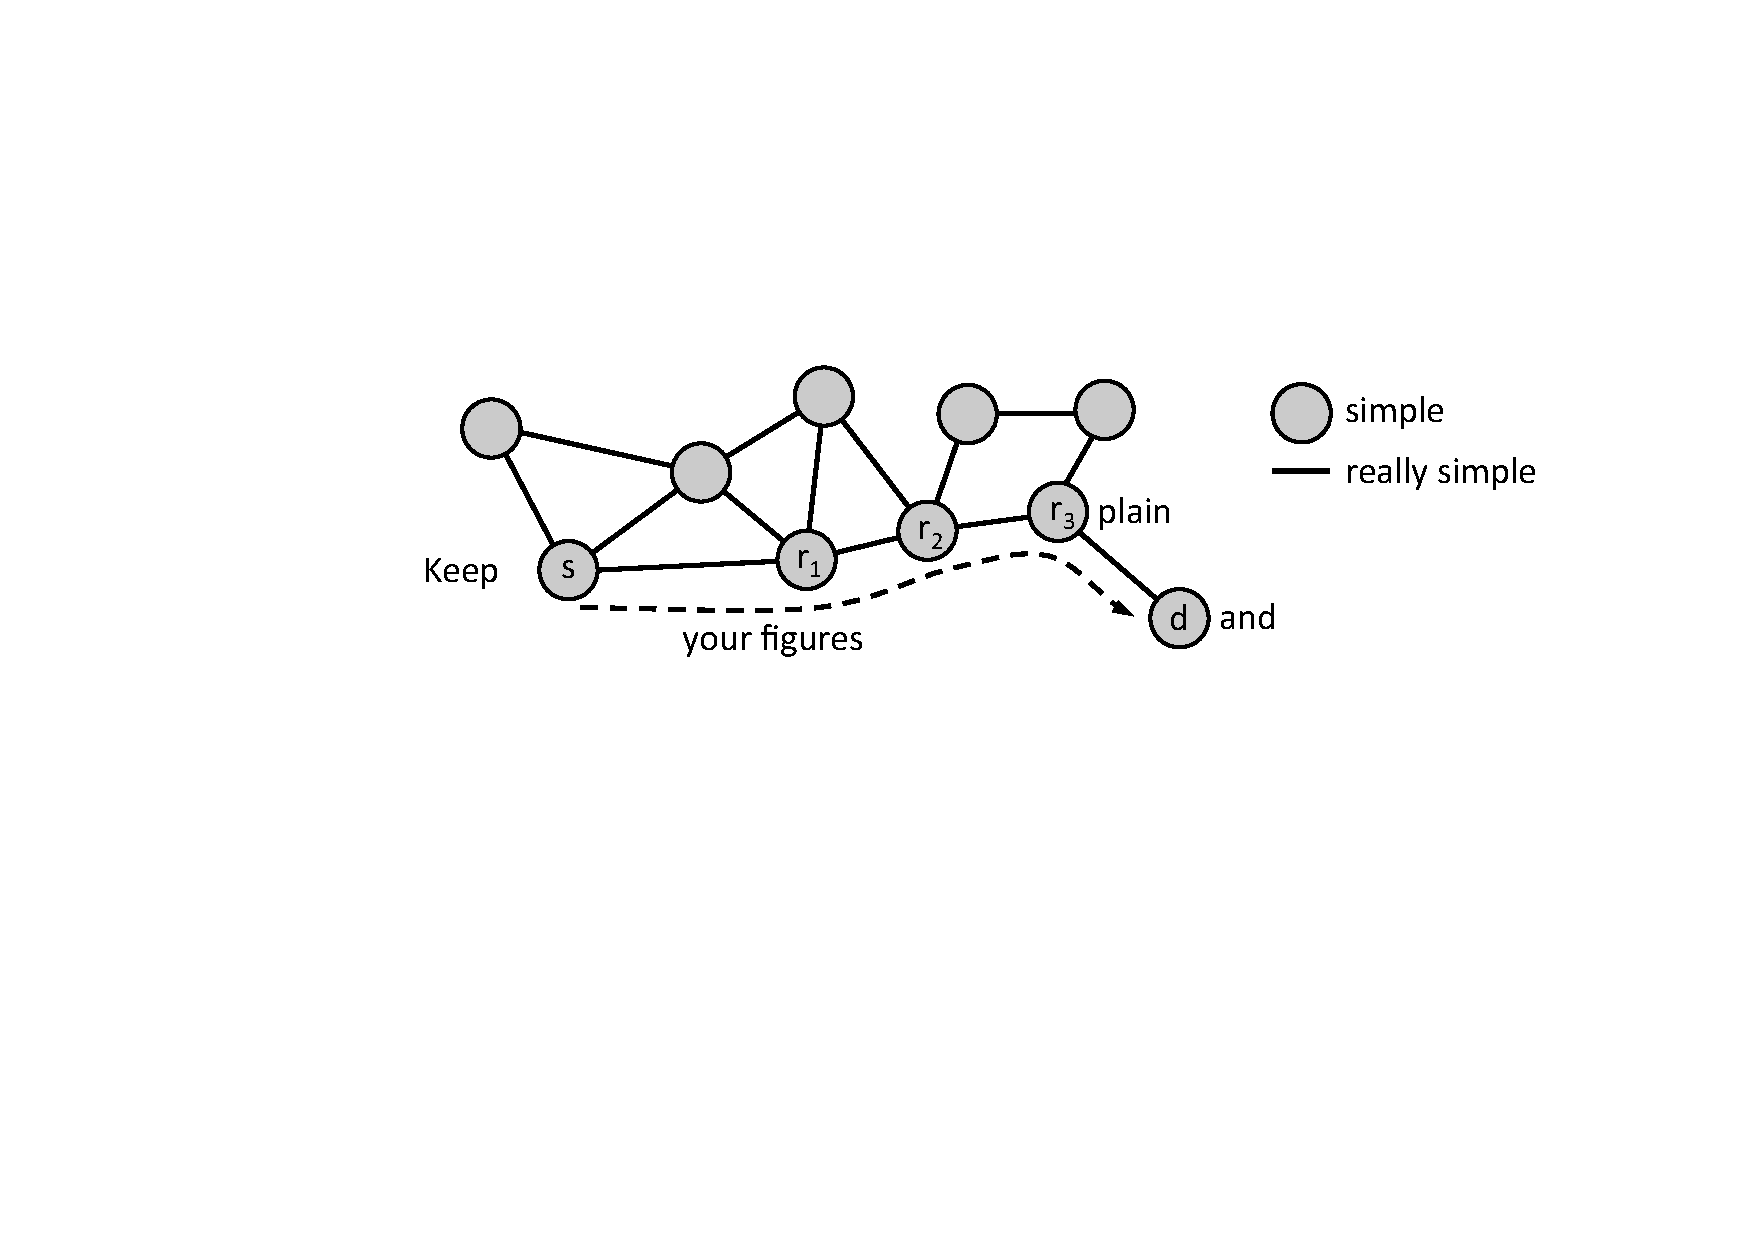
\includegraphics[width=1\columnwidth]{figures/example}
\caption{An example of an awesome image!}
\label{fig:example}
\end{figure} 


Maecenas non tortor lorem, ac cursus nulla. Ut accumsan, felis vitae sollicitudin imperdiet, magna magna semper neque, faucibus feugiat augue neque vel risus. Quisque suscipit pellentesque felis, quis commodo felis mattis et. Maecenas ac augue sed enim posuere facilisis. Nam fringilla faucibus blandit. Morbi ante nisi, sodales in laoreet eu, fermentum sit amet tellus. Integer vel lorem turpis, eu commodo augue. Etiam vel tellus velit, et hendrerit magna. Nulla vitae tellus ut odio pellentesque varius eu eget turpis. In eros neque, rhoncus ac imperdiet eu, luctus eget mi.

Nulla sed lectus pulvinar tellus pretium dignissim pretium in dolor. Sed mollis ornare nisi. Nulla facilisi. Sed porta venenatis ultrices. Sed ut libero nec arcu lobortis suscipit non eget lacus. Donec egestas lacinia ligula, quis tristique eros dapibus eget. Suspendisse iaculis felis id lacus vestibulum malesuada. In vel tincidunt dui. In sed sapien nulla, sit amet venenatis felis. Integer quis leo ipsum, ac sagittis nibh. Curabitur interdum, turpis eu tincidunt ornare, arcu justo aliquet est, ut congue tortor dolor eget leo. Morbi viverra iaculis porttitor. Maecenas eleifend varius tellus, id ultricies sem dapibus id. Fusce lacinia arcu ac odio varius ac ultricies erat mollis. Lorem ipsum dolor sit amet, consectetur adipiscing elit. 

\begin{description}
\item[Ut ac ipsum:]
Ut ac ipsum at velit malesuada tincidunt ornare at sapien. Aenean at dui dolor. Pellentesque sit amet fermentum lorem. Nullam pulvinar diam eget diam hendrerit condimentum. Duis fermentum vulputate ante, a egestas mauris vehicula at. Quisque convallis vestibulum fermentum.

\item[Aenean lacinia elementum:]
Aliquam sed ante id velit ultricies condimentum. Aenean lacinia elementum lacus sit amet luctus. Vestibulum consequat nibh et tortor laoreet sit amet vehicula orci venenatis. Suspendisse enim velit, hendrerit quis vestibulum sit amet, tincidunt sit amet odio.

\item[Phasellus id:]
Nullam ut est lacinia est auctor consectetur faucibus nec tellus. Phasellus id tincidunt risus. Nulla volutpat quam vel diam vehicula in egestas ligula laoreet. 

\end{description}

In consequat laoreet blandit. Ut ac ipsum at velit malesuada tincidunt ornare at sapien. Aenean at dui dolor. Pellentesque sit amet fermentum lorem. Nullam pulvinar diam eget diam hendrerit condimentum. Duis fermentum vulputate ante, a egestas mauris vehicula at. Quisque convallis vestibulum fermentum. Aenean molestie dictum libero, a tincidunt lectus vestibulum in. Vivamus consequat purus pellentesque urna elementum consequat. Cras nec tortor felis, ac cursus risus. Morbi gravida ligula nec orci aliquam aliquam. Morbi et ligula diam, vel venenatis eros. Duis rhoncus ultricies mollis. Nullam ut est lacinia est auctor consectetur faucibus nec tellus. Phasellus id tincidunt risus. Nulla volutpat quam vel diam vehicula in egestas ligula laoreet. 

\begin{table}[b]
\caption{Tables should look like this (save for the last row). If you know LaTeX better than me, feel free to improve the way of producing these tables.}
\begin{tabularx}{\linewidth}{|l|X|X|}
\hline
\rowcolor{slightgray}
\T Tables	&have gray  &headlines\\
\hline
\cellcolor{slightgray}\T and gray &labels \B&, too.\\
\hline
\cellcolor{slightgray}\T T &and B& are used for spacing\B\\
\hline
\cellcolor{slightgray} without T & and B& the cells are too small\B\\
\hline 
\end{tabularx}
\label{tab:example}
\end{table}

Lorem ipsum dolor sit amet, consectetur adipiscing elit. Vestibulum posuere vehicula lorem id commodo. Nam tempor felis quis orci tincidunt suscipit. Morbi dictum purus et nisl porttitor fringilla. Quisque feugiat, tellus quis semper placerat, lectus eros rutrum ipsum, eu elementum nibh nulla eu purus. Vestibulum ultrices varius orci, vitae porta elit laoreet at. Phasellus luctus aliquam molestie. Praesent varius blandit felis eu pellentesque. Aliquam erat volutpat. Morbi at est nibh.

Sed a mi tellus, id pellentesque neque. Integer vel volutpat diam. Sed nec lorem eu arcu lobortis porta. Sed quam nunc, luctus quis facilisis nec, aliquet nec mauris. Mauris non velit nisi, sed convallis risus. Sed quis lectus ligula. Morbi in nibh elit. Aenean a purus justo. Suspendisse pretium semper faucibus. Proin dictum, justo quis sagittis cursus, erat massa sollicitudin magna, in tempus quam lacus non turpis.

Cum sociis natoque penatibus et magnis dis parturient montes, nascetur ridiculus mus. Etiam congue magna at est pellentesque nec hendrerit arcu aliquet. Vivamus sem lectus, vehicula elementum accumsan iaculis, condimentum a mi. Proin sit amet justo eleifend massa eleifend lacinia. Mauris nibh nisl, vehicula vel tincidunt ac, varius et odio. Aliquam feugiat nulla ac felis interdum sodales. Etiam mollis arcu et mi scelerisque quis viverra est vestibulum. Mauris at massa libero, sit amet tincidunt elit. Mauris tempor lorem ut purus hendrerit non viverra nisi vehicula.

Vivamus ligula dui, semper sed consequat non, tempor ut diam. Morbi metus nisl, adipiscing feugiat malesuada viverra, blandit id nunc. Aliquam sed ante id velit ultricies condimentum. Aenean lacinia elementum lacus sit amet luctus. Vestibulum consequat nibh et tortor laoreet sit amet vehicula orci venenatis. Suspendisse enim velit, hendrerit quis vestibulum sit amet, tincidunt sit amet odio. Sed gravida tellus in nunc egestas porta. Morbi suscipit, dui vel elementum volutpat, lectus nulla elementum lacus, vitae dictum erat turpis ut ligula. Donec sit amet dolor ut urna vestibulum consequat nec et purus. In adipiscing lacus vel tellus fermentum quis cursus sapien egestas. Curabitur id ipsum erat. In lacinia adipiscing sapien at varius.

In consequat laoreet blandit. Ut ac ipsum at velit malesuada tincidunt ornare at sapien. Aenean at dui dolor. Pellentesque sit amet fermentum lorem. Nullam pulvinar diam eget diam hendrerit condimentum. Duis fermentum vulputate ante, a egestas mauris vehicula at. Quisque convallis vestibulum fermentum. Aenean molestie dictum libero, a tincidunt lectus vestibulum in. Vivamus consequat purus pellentesque urna elementum consequat. Cras nec tortor felis, ac cursus risus. Morbi gravida ligula nec orci aliquam aliquam. Morbi et ligula diam, vel venenatis eros. Duis rhoncus ultricies mollis. Nullam ut est lacinia est auctor consectetur faucibus nec tellus. Phasellus id tincidunt risus. Nulla volutpat quam vel diam vehicula in egestas ligula laoreet. 

Maecenas non tortor lorem, ac cursus nulla. Ut accumsan, felis vitae sollicitudin imperdiet, magna magna semper neque, faucibus feugiat augue neque vel risus. Quisque suscipit pellentesque felis, quis commodo felis mattis et. Maecenas ac augue sed enim posuere facilisis. Nam fringilla faucibus blandit. Morbi ante nisi, sodales in laoreet eu, fermentum sit amet tellus. Integer vel lorem turpis, eu commodo augue. Etiam vel tellus velit, et hendrerit magna. Nulla vitae tellus ut odio pellentesque varius eu eget turpis. In eros neque, rhoncus ac imperdiet eu, luctus eget mi.

Nulla sed lectus pulvinar tellus pretium dignissim pretium in dolor. Sed mollis ornare nisi. Nulla facilisi. Sed porta venenatis ultrices. Sed ut libero nec arcu lobortis suscipit non eget lacus. Donec egestas lacinia ligula, quis tristique eros dapibus eget. Suspendisse iaculis felis id lacus vestibulum malesuada. In vel tincidunt dui. In sed sapien nulla, sit amet venenatis felis. Integer quis leo ipsum, ac sagittis nibh. Curabitur interdum, turpis eu tincidunt ornare, arcu justo aliquet est, ut congue tortor dolor eget leo. Morbi viverra iaculis porttitor. Maecenas eleifend varius tellus, id ultricies sem dapibus id. Fusce lacinia arcu ac odio varius ac ultricies erat mollis. Lorem ipsum dolor sit amet, consectetur adipiscing elit. 

These are reference and cite examples. See Figure~\ref{fig:example}, Table~\ref{tab:example}, and Listing~\ref{lst:example}. Cite early and often~\cite{exampleentry} is a good rule of thumb.

\chapter{Background}
General discription of used terms/systems in wikipedia like style. This means the description should not be too extensive.
And refer to further papers for more extensive descriptions.
\section{Wireless Networks}
  \subsection{WLAN Channel}
    %https://de.wikipedia.org/wiki/Wireless_LAN#Frequenzen\newline
    \begin{description}
    \item[What is a Channel?]
    \item[Overview on useable frequencies]
    \item[Interference]
    \item[Hidden Station Problem]
    item[\ac{CSMA/CD}]
    \item[Analogy switch - collision domain]
    \end{description}
  \subsection{Wireless Access-Point}
    %Used to establish wireless connections to devices, like laptops/mobile phones, but also printer and ... 
    %Connecting wired LAN - wireless LAN \newline
    %Mostly provide access to internet\newline
    %Usecases of Accesspoints\newline
    %https://de.wikipedia.org/wiki/Wireless_Access_Point \newline
  \subsection{Wireless Mesh Network}
    %https://de.wikipedia.org/wiki/Ad-hoc-Netz
    %Topology for nodes(devices) in a wireless network.
    %Self healing capabilities.
    %Role of Mesh routers.
    %Redundancy in mesh networks.
    %Autonomy of devices.
    %Infrastructure mode vs p2p mode
    %IEEE 802.11
    %Alterations in our scenario compared to standard mesh\newline
    \cite{Akyildiz2005445}
    \cite{airberry}
    \subsection{Wireless Distribution System}
    %https://en.wikipedia.org/wiki/Wireless_distribution_system
    Description of WDS + AutoWDS \newline
      \begin{description}
       \item[What is a Wireless Distribution System?]
       How does the Lancom \ac{AutoWDS},differ from the basic WDS definition?
	 Intended centralized solution compüared to WDS systems due to better managability.
	 Also security is a key element for this system => that's why central entity + CAPWAP
      \end{description}
      \subsection{VLAN}
      \subsection{Spanning Tree + STP}
      \subsection{bandwidth}
      \subsection{BFS}
      \subsection{OpenVZ}
	\cite{openvz}
      \subsection{k-connectivity, k-edge-connectivity}
      \subsection{SSID/ESSID}
\section{Graph-theoretic Basics}
  Since we are using a graph based approahc in finding a solution we model a \ac{WMN} to a graph with a vertex set and an edge set. The goal is then to assign channels
  to the edges of this graph.
  %https://de.wikipedia.org/wiki/Graph_%28Graphentheorie%29
  TODO: Describe directed/undirected weighted graph
  What does connected graph mean; path
   \subsection{Mapping Data to Graph}
    For our solution we will use the following mapping from devices and modules to a undirected, weighted graph. (Formale beschreibung hilfreich?)
    Each accesspoint and each module of those accesspoints is represented by a node.
    For each accesspoint we add edges with the highest weight to each module of its corresponding accesspoint. 
    We describe those edges as artificial or device-module edges.
    If two modules of different accesspoints are within receive range of each other, 
    we are adding an edge between the corresponding module nodes with the average signal-to-noise ratio as the edge-weight.
    We call those edges module-module connections or real connections.
    Since the average of the two SNR's might not adequately represent the actual quality of those connections,
    we alternatively can easily adjust the edge-weight to the minimum or maximum of those values.
    While the average seems to be a good compromise for a general description of the underlying network, the minimum might be a better representation for 
    a more pessimistic setup, since the connection is then guaranteed to have at least this SNR in both directions. 
    Furthermore we are ignoring onesided connections, i.e. one module receives one or a few beacons of the other module but not the other way round.
    Not only are the SNRs of those connections mostly very poor, but they are also very rare in our target scenarios with omnidirectional antennas.
    So mostly either the modules receive each others beacons, or both do not.
    \begin{figure}[t]
      \centering
      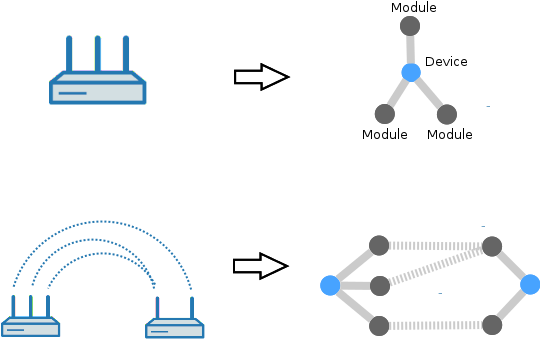
\includegraphics[width=0.5\columnwidth]{figures/apgraph.png}
      \caption{Graph representation of one and two connected accesspoints}
      \label{fig:apgraph}
    \end{figure}
   \subsection{Relevance of COLORING}
   \subsection{Dijkstra's Algorithm}
   TODO: How is our Channel assignment related to the problem COLORING?
    It is realated in the way that we want to assign each Module-Module-Connection a channel/color from a pool of available colors, withouth (if possible) use the same channel/color on neighboring links (meaning Aps that see each other and their traffic could lead to decreased throughput due to interference)
    Why is it not just coloring?

\chapter{Requirement Analysis}
  Up to now AutoWDS automatically uses just one or a random set of channels for its backbone wireless connections. 
  Additionally the topology it creates often reassembles a tree like structure, since the APs connect themselves 
  to the first AP that comes into range and there is no fallback, if a link fails. This results not only in huge bottlenecks for throughput,
  it also leads to greater downtimes if a link happens to fail. Although the APs automatically rejoin the network if possible, it takes
  a considerable amount of time until they are fully reconnected. This is somehow undesirable for the Systems that use this AP as an uplink connection to
  the network. The following requirements for an improved Version of AutoWDS are supposed to tackle those shortcomings.
  \begin{figure}[t]
    \centering
    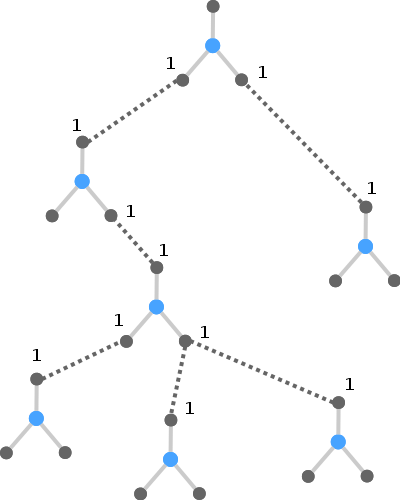
\includegraphics[width=0.3\columnwidth]{figures/autowds_basic_graph}
    \caption{AutoWDS basic network topology and channel assignment}
    \label{fig:autowds_basic_graph}
  \end{figure}
General answer to question of feasibility
  \section{Increase Throughput}
  Since the systems which are connected to the accesspoints consume more data every day and with an increasing storage-footprint of new media like streaming HD videos
  and generally downloading files of up to Gigabytes, a Wireless system is often solely defined by its capability shoveling data over the air to the clients.
  This greed for throughput is amplified by an increasing number of devices that take part in radio communication, 
  thus it is also the key metric for quality in AutoWDS. Furthermore not a single stream of data should be granted exclusively access to the radio, but
  many streams in parallel are desired.
  \section{Reduce Network Connectivity Failures}
\section{Utilize variable Number of Radios}
  Should utilize multiple Radios per AP\newline
  Currently homogenous 2, Later 3, sometimes just 1 \newline
  Also should be able to handle heterogenous environments with respect to number of equipped radios \newline
  \section{Capability of using variable channels}
  Not just fixed amount, but depending on the usecase, like: only 1 and 11 or only 36,40,44
  \section{Restrictions}
  \subsection{Centralized Computation}
    Run on central entity (WLC), not distributed \newline 
  \subsection{Static Environment}
    System is only used for static environments (APs are not mobile) \newline
\section{Economical Restrictions}
  Ressource restrictions (Processing Power limited) \newline
  Duration (Results have to be available in limited time) \newline

\chapter{Related Work}
  The following four approaches are all solutions that are graph-based and target a centralized and static channel assignment.
  Those are not the only ones on this matter, but the approaches currently in use and most relevant contestants to solve our problem.
  Note that there are also numerous solutions on distributed and/or dynamic or semi-dynamic environments, which we will not cover here (See Chapter \ref{reqana}).
  Except the \ac{BFS-CA}, the prevalent solutions make excessive use of the conflict graph, which according to Si et al. \cite{overview_caa} has difficulties to model 
  the varying number of radios equipped on APs. Also, most of the works solely focus on assigning channels to an existing topology and do not touch 
  the network topology at all, what seems like a handicap as topology control is an essential part in dealing with wireless interference as we will see later.
  
  \begin{figure}[h!]
    \centering
    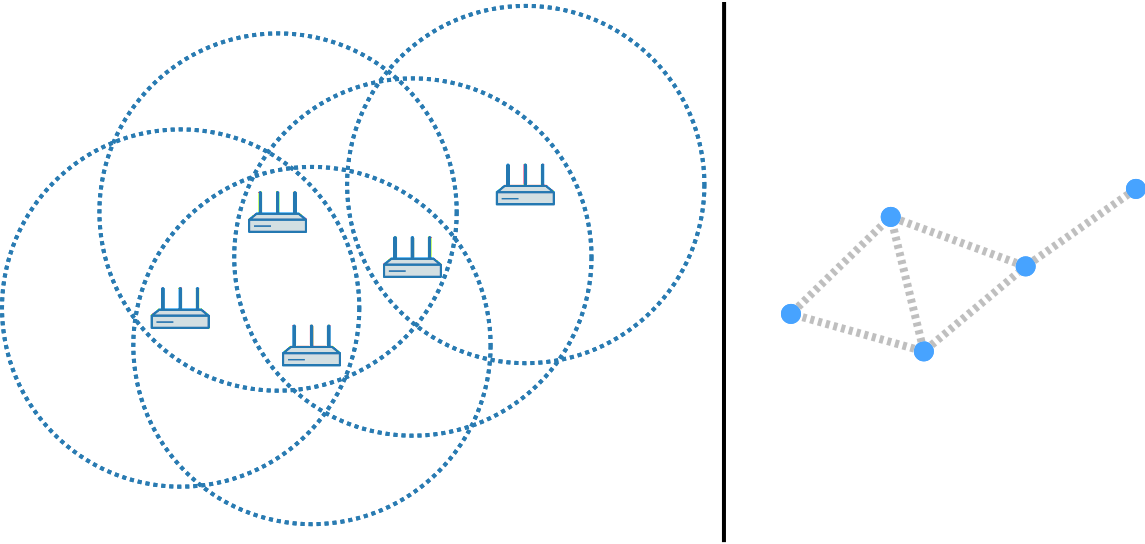
\includegraphics[width=1\columnwidth]{figures/unit-disk-graph}
    \caption{Creation of an unit disk graph from the receive range map of APs}
    \label{fig:unit-disk-graph}
  \end{figure}
  
  \section{\ac{CLICA}}
    The aim of \ac{CLICA} \cite{CLICA} is to minimize interference conflicts for a given unit disk graph preserving the connectivity.
    That means it takes the given network topology-graph as granted and tries to minimize the overall interference by resolving conflicts as much as possible.
    It takes the following parameters as input:
    
    \begin{itemize}
      \item Unit disk graph
      
      \item Number of radios at each node and total number of channels available
      
      \item Interference conflicts in form of a conflict graph
    \end{itemize}
    
    CLICA's mode of operation is described by Si et al. \cite{overview_caa} as follows:
    \begin{itemize}
      \item Randomly assign a node \(v\) the highest priority, then assign other
	nodes priorities decreasing in the order obtained by depth.
	
      \item While traversing the nodes in the decreasing order of their
	priorities obtained above, assign channels to the incident links
	of these nodes. The operation of assigning a channel to a link
	includes assigning this channel to both, a radio at this node and
	a radio at the neighbor node. Then, the priorities of unvisited
	nodes are adjusted according to their degree of flexibility, which
	is the number of channels that a node can choose from without
	breaking the connectivity preservation. Essentially, the nodes
	with a lower degree of flexibility will have their priorities
	increased so that they are visited earlier in the later steps.
	
      \item When picking a channel in the above step, a node \(v_1\) picks
	a channel for its incident link (\(v_1\), \(v_2\)) in a greedy manner: a
	locally optimal choice is made by selecting the channel that
	minimizes the maximum link-conflict-weight among all links
	that can interfere with link (\(v_1\), \(v_2\)). After a channel is assigned
	to a link the conflict graph is updated to reflect the new link conflict weights.
    \end{itemize}
  
    The reason why we decided not to use this algorithm is that \ac{CLICA} only tries to minimize interference by assigning channels the best way possible for a given
    unit disk graph, which is basically each possible connection. For a highly connected network topology like in Figure \ref{fig:graphseen} this would lead to suboptimal results
    as it does not restrict itself to necessary connections and therefore possesses a lot of potential for interference.
    The restriction to use only the best and absolutely necessary links is a vital part in order to 
    further decrease interference as much as possible for such a topology.
    
  \section{\ac{INSTC}}
    As pointed out by Si et al. \cite{overview_caa}, \ac{INSTC} \cite{INSTC} is similar to \ac{CLICA} \cite{CLICA} with a some alterations, 
    which is why we will not go into further detail and rather focus on its differences. 
    They introduce \ac{LCI}, which for a link represents the number of links which interfere with this link and serves as a measure of 
    interference. Additionally, they accept \(k\) as an input parameter which results in a \(k\)-connected graph as outcome to make the topology resilient to node failures.
    Although this feature would come in handy for our survival path requirement, it does not match our failing scenario of a single link at a time instead of a whole node outage.
    Using a \textit{k}-(node)-connected graph instead of an \textit{k}-edge-connected graph increases the number of edges that have to be utilized 
    (since one failing node involves multiple failing edges). Consequently the resulting network topology has a higher grade of connectivity than it needs to 
    have and therefore conversely affects overall throughput since a higher node connectivity leads to fewer usable different channels. 
    Additional to the weaknesses of \ac{CLICA}, they also require the number of radio modules to be identical on each \ac{AP}, 
    which is a deal-breaker for us as we have to be able to fulfill requirement \ref{utilvarnumradio} (Utilize Variable Number of Radios).
    The \ac{LCI} measure introduced here served as a basis for our edgescore calculation in Formula \ref{eq:edgescore}.
    
  \section{\ac{BFS-CA}}
    \ac{BFS-CA} \cite{BFS-CA} extends the common conflict graph with modules, resulting in a \ac{MCG}, which more closely reassembles the
    real world setup. This makes it easier for them to deal with the different numbers of radios available on each device. 
    They let the APs (or mesh routers in their case) sniff the network on regular intervals and determine a ranking for the channels.
    Those rankings are then sent to their central entity, the \ac{CAS}. This \ac{CAS} in turn derives the \ac{MCG} and assigns each node in this graph 
    a channel in \ac{BFS}-manner by considering the received rankings of the APs. In order not to partition the network by introducing a \ac{CA}, which 
    would disconnect some links by setting certain radios to different channels, they also use one radio on each AP on an overall-common channel.
    This common channel is then used for initial setup, management frames and as a backup if other links break in order to keep the graph connectivity attribute.
    
    Although \ac{BFS-CA}, as others, is still anxious about topology alterations, since at a first glance it might introduce too severe problems like, 
    additional hops for packets, increased interference footprint and higher susceptibility to errors due to longer travel times of packets.
    Nevertheless it is the algorithm which we were inspired by the most and therefore have some ideas in common.
    The interesting features we reused and refined are:
    
    \begin{itemize}
     \item Idea of a ranking system for each possible channel
     
     \item Central computation on a \ac{CAS}, which reassembles our \ac{WLC}.
     
     \item Taking foreign sources of interference into consideration as well.
     
    \end{itemize}
    
\newpage
    
    Yet, we decided against its implementation for our purposes for the following reasons:
    
    \begin{itemize}
      \item Using all possible channels in the network topology creates to much interference for networks with more traffic.
	A selection process on this underlying topology is essential to our minds as selecting a few but high quality links
	leading to a planned and controlled topology will create a lot less interference than a network topology where all possible 
	links are used for communications. This is especially the case if not enough channels are available for assignment, since 
	these can be more effectively designed (See Chapter \ref{fig:high_con_vs_low_con}).
	\label{topologypreservingdealbreaker}
	
      \item Using one radio on each \ac{AP} for a common overall-channel seemed to us as a misspending of radio modules.
	Radio modules on APs are scarce and should be utilized efficiently. 
	Furthermore one overall-channel which is utilized by each \ac{AP} does not scale well and is basically already done in \textit{AutoWDS basic}.
	
      \item The ranking process suggested to run on the APs creates load on the APs.
	We want to use the APs merely as sensors and not as decision-makers, 
	since this puts additional load on the APs and brings problems/complexity with synchronisation and
	acquiring the overall view on the network.
	
      \item The ranking algorithm itself could be improved. 
	The solution averages values too early in the process and uses a random pick not as a last resort - providing supoptimal results.
	
      \item \ac{BFS}'s order of assigning channels puts one node (gateway-node) above all others during channel assignment.
	In some of our usescases there is no gateway node available (See Section \ref{reqincreasethroughput}) and we need a fair distribution of channels, 
	which is not feasible with this solution \cite{overview_caa}.
    \end{itemize}

  \section{\ac{CTA}}
    Subramanian et al. \cite{CTA} use a modified Tabu-algorithm \cite{tabu} in two steps to find a \ac{CA} for the conflict graph.
    It works by starting with a random \ac{CA} and, like an evolutionary algorithm, 
    iteratively changing small details and selecting the best temporal solution to continue for the next iteration.
    An iteration is here further subdivided into generating a number of random neighboring assignments, where only the color/channel of one vertex is changed.
    From this set they then select the assignment with the lowest interference.
    The tabu-list, which describes the forbidden options which are not allowed to be chosen for improvement, contains a list of vertex-colorings that already have been used.
    This procedure is then executed as long as there have been improvements in the last \textit{$i_{max}$} rounds.
    If for \textit{$i_{max}$} rounds no improvement can be found, the algorithm proceeds with step two.
    As the first step may give channel assignings which are not valid (more channels assigned than a node has radios), the second step merges channel assignments 
    until the solution is valid again. Merging channels obviously increases the interference.
    
    This solution is also topology preserving and a deal-breaker for our implementation (See Section \ref{topologypreservingdealbreaker}).
    Additionally the evolutionary attribute does not provide controlled, but more heuristic results and we need an algorithm with more control over its internals.
\chapter{Algorithmic Design}
  Even for a simple scenario like in Figure \ref{fig:graphseen},
  where we have a lot of possible links between the modules it is not obvious how to chose a low-interference network topology from this graph.
  A shortsighted solution may be trying to use every possible link, 
  since this would decrease overall travel times for each packet and therefore reducing network workload and possible interferences as a packet is not longer in the network than it needs to be. 
  The problem in doing so is the small number of channels we can assign to these links, even if we allow using multiple channels.
  Since we can only assign one channel to a module, trying to start small and assigning one channel to one module would then force us to also 
  assign the same channel to all connected modules in order to maintain connectivity as two modules can only communicate with each other if they use the same channel
  (See upper half in Figure \ref{fig:high_con_vs_low_con}). 
  
  \begin{figure}[h!]
    \centering
    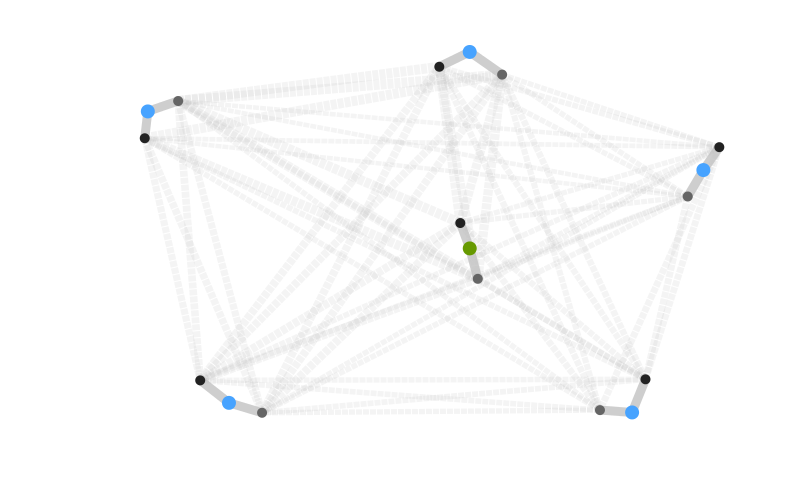
\includegraphics[width=0.8\columnwidth]{figures/graphseen.png}
    \caption{Network topology graph for a simple scenario with 6 APs / 2 modules each. The green node indicates a connection to wired network.}
    \label{fig:graphseen}
  \end{figure}

  \begin{figure}[h!]
    \centering
    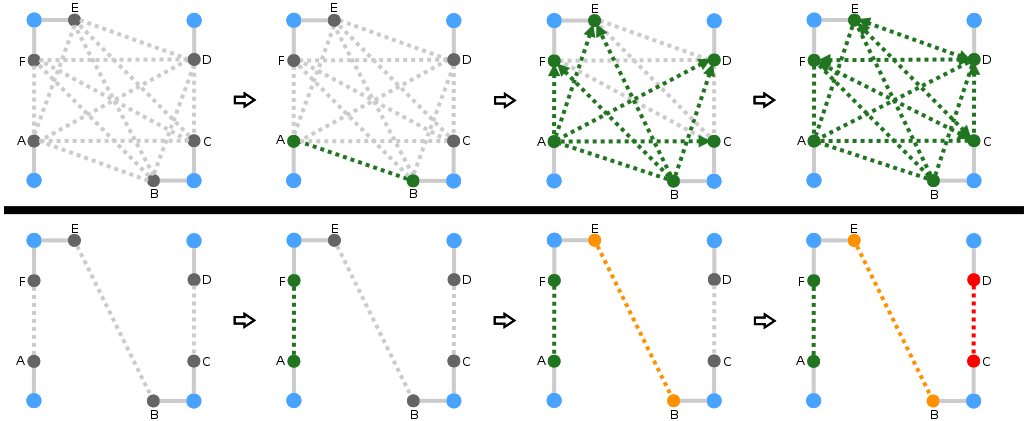
\includegraphics[width=1\columnwidth]{figures/high_con_vs_low_con.png}
    \caption{Coloring a highly connected network (upper) may result in fewer channels with high interference being used compared to 
      a reduced network topology (lower) where multiple interference-free channels can be used.
      Especially the dependent modules, which also have to receive the same channel in order to maintain connectivity are the reason for single channel usage here: 
      Wanting to only color edge A, B you also have to assign the same channel to nodes C, D, E, F and therefore its edges.}
    \label{fig:high_con_vs_low_con}
  \end{figure}
  
  On the other hand if we chose a small subset of links in this graph(like a \ac{MST}), we might be able to assign more channels, 
  leading up to no interference at all (See Figure \ref{fig:high_con_vs_low_con}).
  As a drawback this could create bottlenecks, single points of failures and leading to packets staying longer in the 
  communication network since they can not take the shortest path.
  This is why we later need to add further links (survival paths).
  
  A consequence of the mono-channel setup in a dense topology is a radical throughput performance loss as a transmission from
  A to B would prohibit any other communication due to the utilization of the same channel.
  Even if links (A, F), (E, B) and (D, C) would have a low link quality and packets can not travel directly to their destination
  a simultaneous transmission allows a higher throughput in the same time.
  Naturally only the second solution is favorable for a bigger scenario, because more APs would have to wait to put their data on the spectrum.
  Especially adding redundant links to a small subset of links in order to fulfill the reduced end-to-end link failure requirement is not straight-forward.
  Each newly added link increases overall throughput capacity, but at the same time may create co-channel interference or worse,
  decrease the number of overall assignable channels.
  
  \begin{figure}[h!]
    \centering
      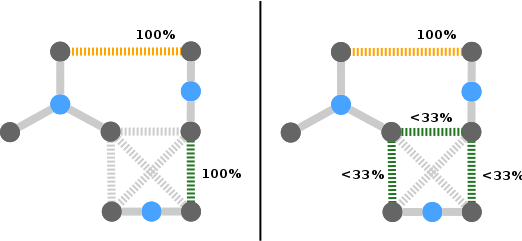
\includegraphics[width=0.8\textwidth]{figures/lessismore}
      \caption{Additional links do not necessarily increase throughput performance rather on the contrary may decrease the number of non-interfering channels used (3 vs 2).
	Percentage depict link quality and therefore flow capacity.}
    \label{fig:lessismore}
  \end{figure}
  
  In the following two sections we will present an algorithm creating network topologies, seeking to find the best compromise,
  by first creating the topology and then assigning channels on the resulting topology as basis.
 
  \section{Topology Creation}
    Creating the topology is also split into two parts.
    First, creating a \ac{MST}, respecting a certain provided formula, which scores edges depending on their expected throughput.
    Second, adding redundancies in form of backup or parallel links to the \ac{MST}. 
    To make it more vivid we added an example after the algorithmic description.

    \subsection{Minimal Spanning Tree Topology}
      In order to select the edges we want to use for creating connections between the APs, we use a derivation of the \ac{DJP}-algorithm \cite{jarnik, prim}.
      The reason we chose a \ac{MST} algorithm over other techniques like all-pairs shortest path is, that a \ac{MST} gives us the best essential edges in a graph. 
      We can then extend these essential set of edges with further redundant edges if we have or want to (survival paths). 
      Adding more than the essential edges immediately plays in favor of interference, which we want to avoid by all means and so have to do so carefully.
      
      From the set of all nodes which are connected by edges, we start by selecting an arbitrary initial node and mark it as visited. 
      All edges from this set of visited nodes to unvisited nodes are called productive edges.
      We keep those productive edges in a list sorted by their scores. The score of an edge is determined by the following formula:
      
      \begin{equation} \label{eq:edgescore}
	ES=\frac{b}{(i + 1 )* (c + 1)}
      \end{equation}
      
      where \textit{ES} is the score of this edge, \textit{b} is the expected bandwidth, \textit{i} is the number of 
      interfering modules and \textit{c} is the connected count of the corresponding nodes. 
      Dividing \textit{b} by \textit{i} and \textit{c} describes how the theoretically available bandwidth would have to be shared among other interfering radios.
      This characteristic results in a lower \textit{ES} for edges where the assumed throughput is lower due to interference by other radios.
      The following three subsections will explain the formula in more detail.
      
      For each round we determine from this list the edge with the highest score.
      If two links have the same \textit{ES} and different SNRs, we pick the edge with the higher \ac{SNR} as this edge has to share its channel
      among fewer participants and therefore results in higher throughput with fewer interference to the network.
      As a last resort if there is also a tie in \ac{SNR} values, we pick one at random.
      We then mark the new node as visited and add also the new links to the list.
      Finally we have to update the scores for each affected link and continue with the next round until all nodes are marked visited.
      The outcome is a minimal spanning tree for this graph with a custom evaluation function.
      
\newpage
      
      \subsubsection{Interfering Modules}
	Since the channel assignment has not taken place yet, we do not know which modules are actually interfering with this link if we would use it.
	However we do know to which other modules this module already has connections to and since those have to use the same channel in order to communicate with each other,
	we can derive an estimate as lower bound for the number of interfering modules for this link (A, B) by counting the following modules:
	Total interfering modules is equal to the number of visited nodes which we can reach by one hop over a module-module connection from node A and B.
	Those modules definitely interfere with our current connection, since they:
	
	\begin{itemize}
	\item are in range with at least one node of this connection (one hop distance)
	\item have to use the same channel (communication over module-module link)
	\item do actually interfere, because we already decided to use this connection (visited node)
	\end{itemize}

	The value is incremented by one, because if this connection would be used, itself again acts as a source for interference and it nicely solves the division by zero problem.
	With an increasing count in interfering modules, the value of the link decreases and vice versa. This reflects perfectly the concept of a shared medium.

      \subsubsection{Expected Bandwidth}
	describes the expected available bandwidth we assume to get for this link depending on the \ac{SNR}.
	For a given \ac{SNR} we can estimate the maximal possible throughput since effective bitrate and therefore throughput is amongst others dependent on the \ac{SNR}
	and modulation which is continuously adjusted by the network driver for the radio module during operation.\footnote{The rate adaptation algorithm 
	which is used in LANCOM devices is Minstrel \cite{minstrel}.} 
	The bandwidth was chosen as the numerator, since it is effectively shared by the radio modules within range.
	
	As we can take from Figure \ref{fig:snr_tp}, a higher \ac{SNR}-value results in more bandwidth available to use and share and works in favor of this edge.
	Note that the mapping of \ac{SNR} to achievable throughput may have to be adjusted for different hardware / devices / drivers. 
	In general the behaviour will stay the same, as a higher \ac{SNR} will necessarily result in a better modulation, which also increases throughput.
	
	\begin{figure}[h!]
	  \centering
	  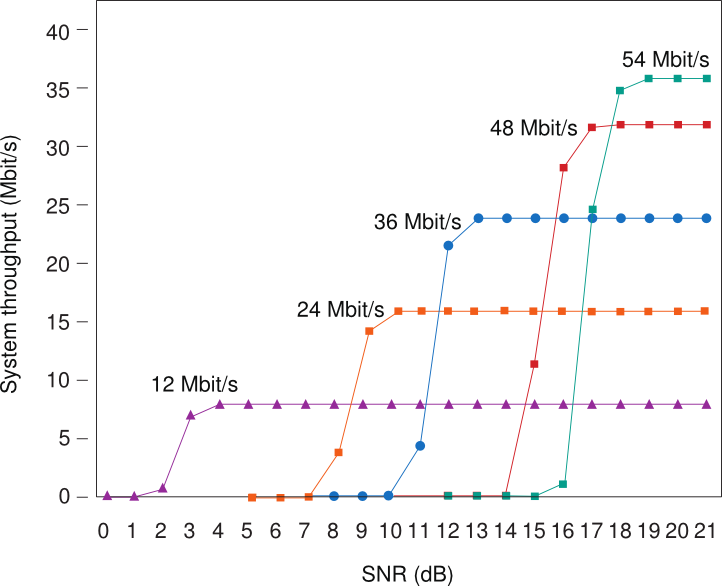
\includegraphics[width=0.6\columnwidth]{figures/snr_tp}
	  \caption{Expected throughput \ac{SNR}-values by Otsuki et al. \cite{expected_snr}.
	    We assume to get the best possible throughput for a given \ac{SNR}, since modulation is automatically adapted by the APs with increasing \ac{SNR}.}
	  \label{fig:snr_tp}
	\end{figure}
	
	Another factor of influence would be the number of erroneous bytes that have been transmitted over this link. 
	This is however not used for determining the expectet bandwidth as we do not know what those values are going to look like before actually using this link to transmit data.

      \subsubsection{Connected Count}
	The number of nodes we can reach from module A and module B by just using module-module edges (For example nodes A, B, C in Figure \ref{fig:channel-list}). 
	A higher connected count diminishes the importance of this edge, since this value controls how many channels we can use later for the overall graph.
	If this value would not be taken into consideration for calculating the score, the algorithm would rather create long chains of connected modules. 
	Those links in this chain would admittedly have the best \ac{SNR} values, but since they have to share the same channel,  
	it would result in lowering the overall throughput.
	Granting this value a higher impact in the formula, like for example in 
	
	\begin{equation}
	  ES=\frac{b}{(i + 1)* (c + 1)^2}
	\end{equation}
	
	would have the effect of overemphasizing the module connectedness and lead to poor choices in links with respect to \ac{SNR} - 
	lowering overall throughput again.
	The simple, linear impact in the formula has shown to achieve the best tradeoff between those two extremes.
	
	\begin{figure}[h!]
	  \centering
	  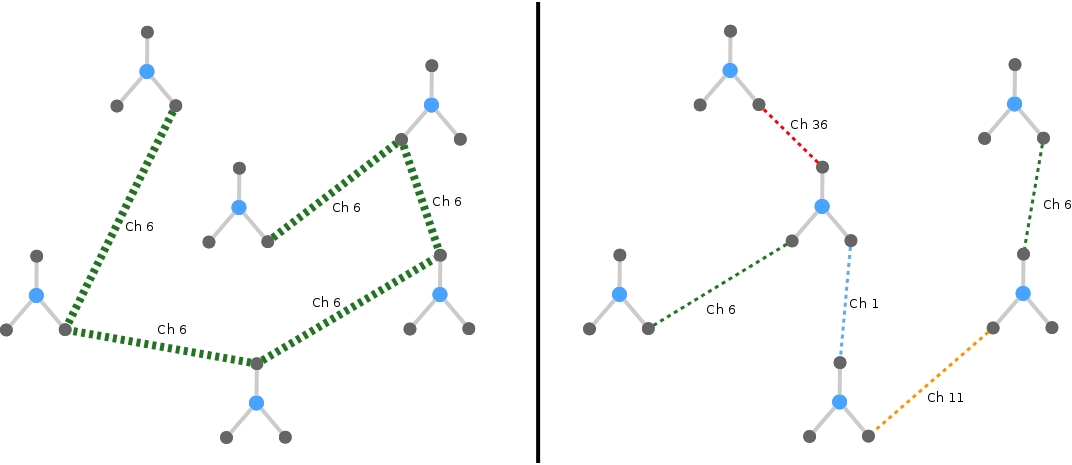
\includegraphics[width=1\columnwidth]{figures/formula_graphic}
	  \caption{Impact of the connected count on the formula. Resulting topology in case the connected count is underemphasized (left) leading
	    to long chains of possibly high quality links, but only one usable channel, which has to be shared among all modules.
	    Topology in case of an overemphasized connected count (right).
	    As the algorithm avoids reutilizing already used modules, links with low quality are preferred,
	    leading a lot of exclusive channels with lower link quality.
	    Thicker edges illustrate better link quality.}
	  \label{fig:formula_graphic}
	\end{figure}

\newpage
	
      \subsubsection{Example MST Creation}
	Let's take a look at a simplified example, where we assume \textit{b=SNR}.
	Also note that we immediately expand module-device edges to keep the example short.
	Normally the algorithm would also expand each of those edges step by step.
	However due to their maximum weight these have precedence over all other edges, so that we merely skip the tedious images.
	\begin{figure}[h!]
	  \centering
	  \begin{minipage}{0.5\textwidth}
	    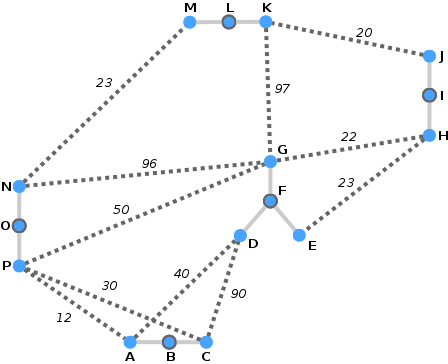
\includegraphics[width=\columnwidth]{figures/mst_calc_1}
	  \end{minipage}
	  \caption{Example input topology - Edge-weights representing the \ac{SNR}}
	  \label{fig:mst_calc_initial}
	\end{figure}
	
	Figure \ref{fig:mst_calc_initial} represents the underlying network topology with all possible links for a scenario with five APs where all APs are equipped with two
	radios except F, which has three.
	
	\begin{figure}[h!]
	  \centering
	  \begin{minipage}{7.4cm}
	    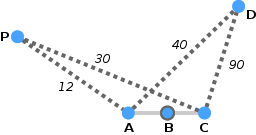
\includegraphics[width=4.5cm]{figures/mst_calc_2}
	  \end{minipage}
	  \begin{minipage}{4cm}
	    \begin{tabular}{c||c|c|c||c}
	      Edge & \textit{b} & \textit{i} & \textit{c} & \textit{ES}\\ \hline\hline
	      (A,D) & 40 & 0 & 0 & 40 \\ \hline
	      \textbf{(C,D)} & \textbf{90} & \textbf{0} & \textbf{0} & \textbf{90} \\ \hline
	      (A,P) & 12 & 0 & 0 & 12 \\ \hline
	      (C,D) & 30 & 0 & 0 & 30 \\ \hline
	    \end{tabular}
	  \end{minipage}
	  \caption{First round - Picking (C, D) with highest score}
	  \label{fig:mst_calc_2}
	\end{figure}
	
\newpage
	
	We start off by selecting a random node (B).
	Actually the first steps here would have been expanding the fake edges (B, A) and (B, C), but as noted above we skip those.
	From this set of nodes we then consider all edges to newly, up to now undiscovered nodes (listed in the right table in Figure \ref{fig:mst_calc_2}).
	From this list of edges we calculate the \textit{ES} on each edge, which results in the selection of edge (C, D). 
	Note, from now on the values on the edges represent the \textit{ES} instead of \textit{b}.
	
	\begin{figure}[h!]
	  \centering
	  \begin{minipage}{7.5cm}
	    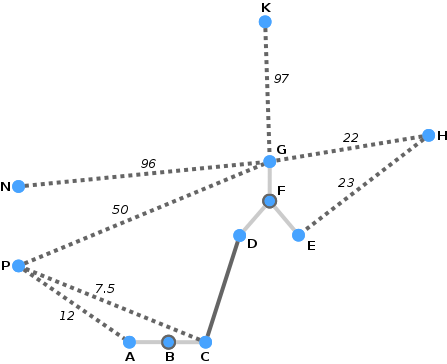
\includegraphics[width=7cm]{figures/mst_calc_3}
	  \end{minipage}
	  \begin{minipage}{4cm}
	    \begin{tabular}{c||c|c|c||c}
	      Edge & \textit{b} & \textit{i} & \textit{c} & \textit{ES}\\ \hline\hline
	      (A,P) & 12 & 0 & 0 & 12 \\ \hline
	      (C,P) & 30 & 1 & 1 & 7.5 \\ \hline
	      (G,P) & 50 & 0 & 0 & 50 \\ \hline
	      (G,N) & 96 & 0 & 0 & 96 \\ \hline
	      \textbf{(G,K)} & \textbf{97} & \textbf{0} & \textbf{0} & \textbf{97} \\ \hline
	      (G,H) & 22 & 0 & 0 & 22 \\ \hline
	      (E,H) & 23 & 0 & 0 & 23 \\ \hline
	    \end{tabular}
	  \end{minipage}
	\caption{Second round - Score for edge (C,P) decreased - Picking edge (G, K)}
	\label{fig:mst_calc_3}
      \end{figure}

      After the expansion of the fake edges for \ac{AP} F, we proceed by refreshing all the edgescores, portraying edge (G, K) as the best edge (See Figure \ref{fig:mst_calc_3}).
      Note how the score for edge (C, P) was decreased, since node C is already used for another edge.
      
      \begin{figure}[h!]
	\centering
	\begin{minipage}{7.5cm}
	  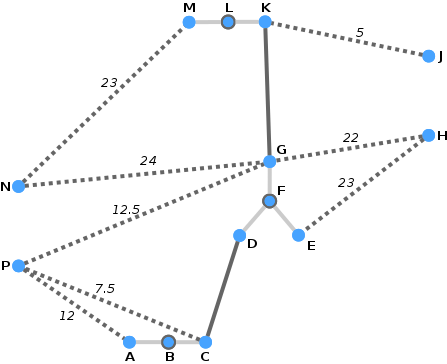
\includegraphics[width=7cm]{figures/mst_calc_4}
	\end{minipage}
	\begin{minipage}{4cm}
	  \begin{tabular}{c||c|c|c||c}
	    Edge & \textit{b} & \textit{i} & \textit{c} & \textit{ES}\\ \hline\hline
	    (A,P) & 12 & 0 & 0 & 12 \\ \hline
	    (C,P) & 30 & 1 & 1 & 7.5 \\ \hline
	    (G,P) & 50 & 1 & 1 & 12.5 \\ \hline
	    \textbf{(G,N)} & \textbf{96} & \textbf{1} & \textbf{1} & \textbf{24} \\ \hline
	    (G,H) & 22 & 1 & 1 & 5.5 \\ \hline
	    (E,H) & 23 & 0 & 0 & 23 \\ \hline
	    (K,J) & 20 & 1 & 1 & 5 \\ \hline
	    (M,N) & 23 & 0 & 0 & 23 \\ \hline
	  \end{tabular}
	\end{minipage}
	\caption{Third round - Best edge is (G,N).}
	\label{fig:mst_calc_4}
      \end{figure}
      
      All edges connected to G have been recalculated as G was used in the last step. Edge (G, N) is nevertheless the edge which promises according to 
      the formula the most throughput, even more than the up to now unused edge (E, H).
      
      \begin{figure}[h!]
	\centering
	\begin{minipage}{7.5cm}
	  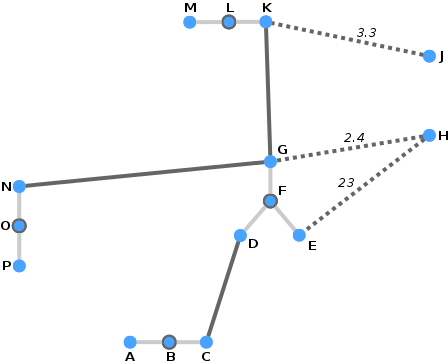
\includegraphics[width=7cm]{figures/mst_calc_5}
	\end{minipage}
	\begin{minipage}{4cm}
	  \begin{tabular}{c||c|c|c||c}
	    Edge & \textit{b} & \textit{i} & \textit{c} & \textit{ES}\\ \hline\hline
	    \textbf{(E,H)} & \textbf{23} & \textbf{0} & \textbf{0} & \textbf{23} \\ \hline
	    (G,H) & 22 & 2 & 2 & 2.4 \\ \hline
	    (K,J) & 20 & 1 & 2 & 3.3 \\ \hline
	  \end{tabular}
	\end{minipage}
	\caption{Fourth and final round - Best edge to connect the last nodes is (E,H)}
	\label{fig:mst_calc_5}
      \end{figure}
      
      Edgescores of the remaining links rapidly decrease as using these would definitely cause interference.
      This is the first step the connected count \textit{c} has a greater impact in calculating the \textit{ES} as the path N, G, K has length two.
      Using edge (G, H) would increase this distance to three,
      which would be unfavourable for the coloring process (all edges connected to G would have to use the same channel).
      Luckily we can utilize (E, H) which does not necessarily interfere with other links (it may interfere after the coloring process, if not enough colors are available).
      
      \begin{figure}[h!]
	\centering
	\begin{minipage}{7.5cm}
	  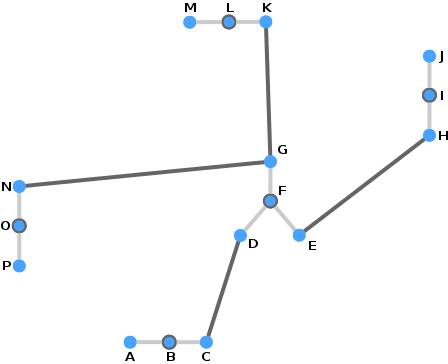
\includegraphics[width=7cm]{figures/mst_calc_6}
	\end{minipage}
	\begin{minipage}{4cm}
	  \hspace{4cm}
	\end{minipage}
	\caption{Resulting MST}
	\label{fig:mst_calc_6}
      \end{figure}  
     \newpage
      
    \subsection{Survival Paths}
      A spanning tree is particularly susceptible to graph partition by just removing one link so we have to add redundancies in form of supplementary connections.
      However those redundant connections have to be carefully chosen in order not to negatively impact the successive channel assignment and therefore to push interference.
      Note that this is an optional feature,
      since for some use cases a spanning tree topology is enough or a topology with redundant links is not easily implemented with the existing code or hardware.  
      
      We accomplish this by iterating over all the edges of the spanning tree and simulate each connection failing. 
      We then check if there still exists a path from node A to node B of this failing connection. 
      Only if this failing connection cuts the graph in half and there is no path to the other side,
      we start looking for a backup route in the following fashion:
      First we separate the graph into two groups: Group A with all nodes and links reachable from node A and group B with the same for node B.
      We create a list with unused edges which connect the two groups and calculate the scores on them and pick again the edge with the highest score.
      This edge is the best edge to reconnect the two parts (according to Formula \ref{eq:edgescore}) and is called the survival edge for this failing scenario.
      Nevertheless we have to be aware that it might not be feasible to reconnect those parts if the underlying structure does not permit it.
      For example the link between nodes \(E\) and \(F\) in Figure \ref{fig:survival_algo} might be the only connection possible and failing it would cause network disruption.
      But if this link fails there is nothing we can do.
      The result is a robust network topology, which despite the added interfering links still yields a high overall throughput with redundant paths.

      The survival path attribute for a graph can also be expressed in the following formal way:
      \begin{quote}
	For each edge (a, b) of the calculated spanning tree graph G', find a path from a to b without traversing (a, b), 
	in a way that the sum of the Edgescores of the path is maximal.
      \end{quote}
      Formally defined as:
      $$\textit{G}=(\textit{V},\textit{E}) \quad
	\forall \textit{edge}_\textit{a,b} \exists \textit{path}_\textit{a,b} | \textit{edge}_\textit{a,b} \notin \textit{path}_\textit{a,b} \quad
	\textit{a,b} \in \textit{V}, \textit{edge}_\textit{a,b} \in \textit{E}$$
	Finding the optimal edge:
	$$\textit{max}(\textit{edgescore}(\textit{path}_\textit{a,b})) |
	\textit{edgescore}(\textit{path}_\textit{a,b})) = \sum_{\substack{e \in \textit{path}_\textit{a,b}}} \textit{edgescore}(e)$$
	
    Using survival path actively and additionally to the \ac{MST} links, instead of a fallback, 
    would require a shortest path routing that deals with circles in the graph.
   
    \begin{figure}[h!]
      \centering
      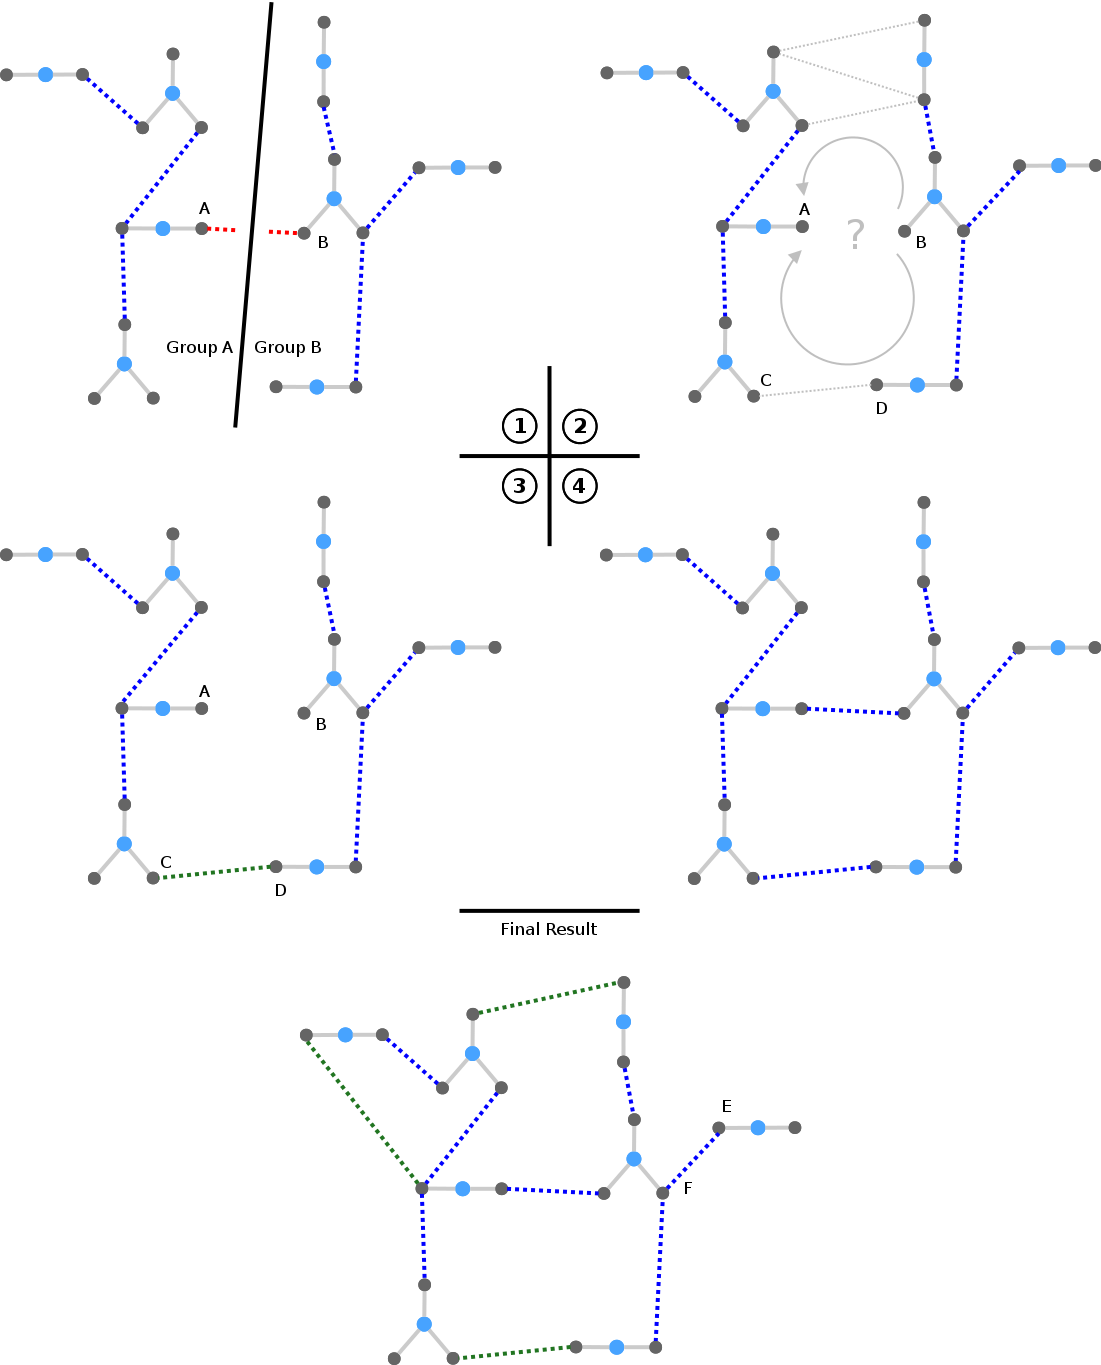
\includegraphics[width=1\columnwidth]{figures/survival_algo2}
      \caption{Finding survival paths. Simulation of connection between node A and node B failing, creating two groups.
	Finding a survival path for node A and B.
	Eventually all connections have a survival path.
	No redundant link possible for failing connection (E, F).}
      \label{fig:survival_algo}
    \end{figure}
    
    \begin{table}[h!]
      \centering
      \begin{tabular}{|c|c|}\hline
	Channel & Interference Count\\ \hline
	36 & 4 \\ \hline
	\textbf{11} & \textbf{1} \\ \hline
	\textbf{1} & \textbf{1} \\ \hline
      \end{tabular}
      \begin{tabular}{|c|c|}\hline
	Channel & Interference Count\\ \hline
	\textbf{36} & \textbf{4} \\ \hline
	11 & 5 \\ \hline
	1 & 5  \\ \hline
      \end{tabular}
      \caption{Channel-list without (left) and with (right) foreign influence}
    \end{table}
    
\newpage
    
  \section{Channel Assignment Algorithm}
    For a given network topology graph and a set of channels to chose from, we can now assign channels to the module-nodes or if you like the links between those.
    Therefore we iterate over all module-module edges and assign channels to the adjacent module-nodes if they do not already have one assigned.
    The channel for an edge is chosen by the following pattern for each channel-group:
    Select all the modules which are connected by module-module edges.
    This set of nodes is called the channel-group.
    For this channel group we create a list of channels and corresponding interference occurrences.
    Among these we pick those channels from the set of all possible channels, which have been used the least in this channel-list.
    If there is a tie in usage we can additionally respect foreign networks by taking the occurrences of foreign radio modules also into account.
    Since we do not know how much traffic the foreign channels carry and therefore how much they utilize the channels,
    we can only weight them equally compared to our own channel-usage instead of a more fine-grained subdivision.
    As a further tie-breaker we pick those channels which have been used the least in general.
    At last we resort to just selecting one channel at random, but this should rarely occur.
    Especially respecting foreign networks allows use to evade heavily used bands and channels like for example 1 and 11 in the 2.4 GHz band which 
    are used by devices out of our control.
    
    \begin{figure}[h!]
      \centering
      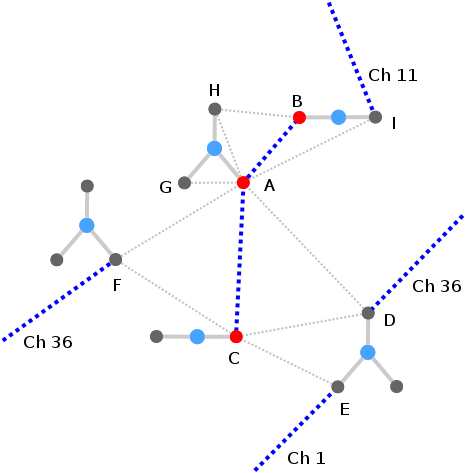
\includegraphics[width=0.7\columnwidth]{figures/channel-list}
      \caption{Channelset A,B,C selected for coloring.}
      \label{fig:channel-list}
    \end{figure}
    
\newpage
    
    Since A, B and C are in the receive range of D, E, F, G, H, I they are possible sources of interference if we use the same channel as those. 
    Therefore we survey how often every channel interferes, where one module can also interfere multiple times.
    For example does module F which already has channel 36 assigned interfere 4 times with the channel-set A,B,C ((A, F), (C, F), (C, D), (A, D)). 
    If we only could choose from channel 1,11 and 36 we would then decide to use channel 1 or 11 to assign to the channel-set depending on how often we overall used those already.
    If however we want to take also foreign networks into consideration and lets say modules A and C would both detect two other \ac{WLAN} networks at channel 11 and two
    at channel 1, then we would add another four for channel 11 and channel 1 in the channel-list, leading to Channel 36 as the best choice. 
    Note modules G and H are ignored for the counting process since they do not have links or channels assigned.
    
    \begin{figure}[h!]
      \centering
      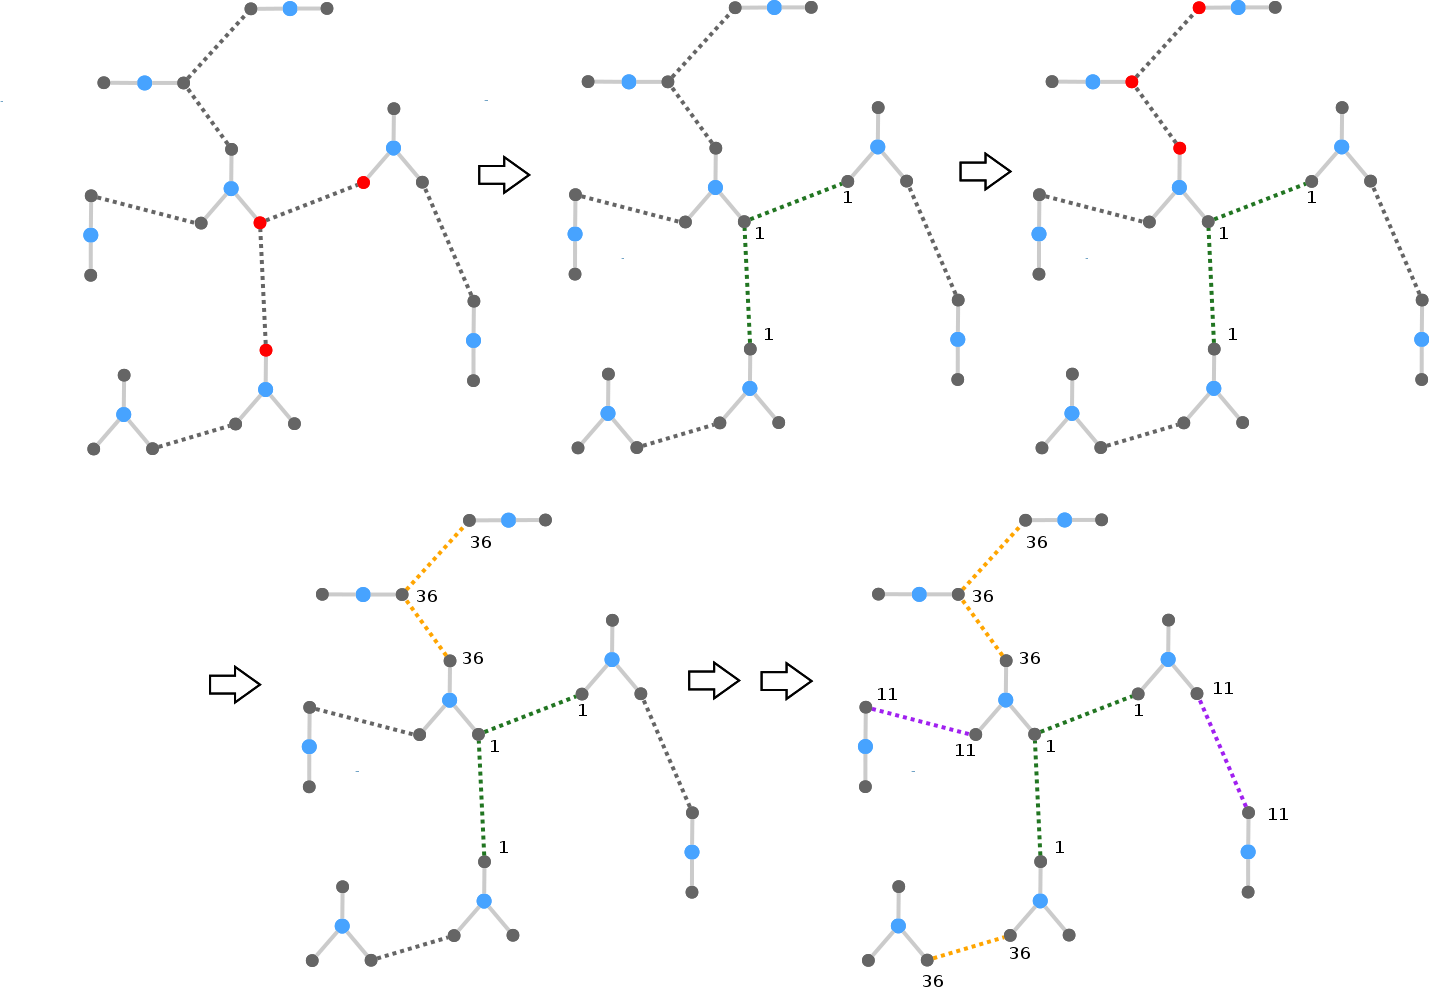
\includegraphics[width=1\columnwidth]{figures/caa_algo}
      \caption{General overview on the channel assignment process.}
      \label{fig:caa_algo}
    \end{figure}

    Figure \ref{fig:caa_algo} shows an example-assignment for a network with 8 APs with 2 and 3 modules equipped and available channels [1, 11, 36] without foreign influence. 
    Each graph depicts the status after each of the assignments. 
    Red marked nodes represent a channel-group. 
    Currently there is no special order in which the channel-sets are colored. 

\chapter{Implementation}
  The language of choice we used for the implementation is python2.7. Although we also could have implemented the extension in c/c++ since the basic version
  was already written in this language, python does have some key advantages we did not want to miss.
  
  \begin{description}
    \item [Rapid prototyping]
    Since our algorithms can easily work on a given set of data completely independent and the interfaces to get the data from are clearly defined and accessible,
    using a lightweight language like python had the benefit of not having to embed our new code into the existing environment. Although it still can be implemented 
    in the native language C/C++ for our scenario, this will take some more time and effort, which was not the focus of this work.
    \item[Existing libraries]
    like NetworkX in python made it particulary easy for us to map real world scenarios to graph abstractions as we did not have to create those structures ourselves.
    Although there are some libraries that provide graph abstractions in C/C++ we could not have as easily employed them due to their copyright restrictions and 
    the closed source virtue of our target system.
    \item[Faster Debugging]
    Especially the initial phase of the project was errorprone and needed a lot of debugging. Not having to recompile after every fix turned out to be
    a great saving of time. Not to mention the live debugging capabilities of python, which was really helpful.
    \item[Existing APIs]
    Fortunately also the code for interaction with the interfaces (SNMP/SSH/Telnet) of the WLC was written in Python, so we could easily 
    integrate it into ours and had no problem gathering the 'seen'-data. Unfortunately for you those libraries are closed source to the public.
    \item[Maintainability]
    As python has the reputation of being an easy to learn language, this was another benefit and played absolutely in our favor with the goal of
    keeping the code simple, lightweight and reuseable by someone else.
  \end{description}
  
  \section{Dependencies}
    As already mentioned we used NetworkX\cite{hagberg-2008-exploring} to model our graphs and work with its elements.
    NetworkX's rich features like ``has\_path'' made things especially easy in computing the survival paths.
    Another library we used is python collections. \cite{python_collections}
    This library implements specialized container datatypes additionally to those shipped with standard python.
    It's `Counter` structure is used to create the channel-lists and retrieve the most or least used elements.
    We extended this library for our convencience since it did only provide the functionality for getting the most common element from its list and not the least common,
    which we needed. \footnote{It is worth mentioning that the request for including this method was already issued at 01/2013 http://bugs.python.org/issue16994}
    The only closed source library we used is the herein before mentioned library to query the WLC for the data of the APs. Nevertheless gathering the data can also
    easily be separated and outsourced to different interfaces.
  
    \begin{figure}[h!]
      \centering
      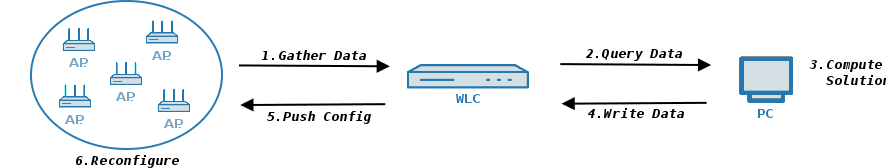
\includegraphics[width=1\columnwidth]{figures/dataflow}
      \caption{General flow of information for our scenario}
      \label{fig:dataflow}
    \end{figure}
  
  \section{Structure of the Code}
    We split the code into two modules. The one handling connections, sending/receiving and transforming data to and from networkX graphs and the other one 
    deals with only with graphs and therefore the theoretical problem.
    
    \subsection{Interfacing Outer World and Managing Data}      
     \begin{table}[h!]
	\begin{tabular}{clll}
	  Device Mac Address & Module Mac Address & Seen Module Mac Address & \ac{SNR}\\ \hline
	  ece55574a4d5 & ece555ffd61e & ece555ffd5bf & 56 \\
	  ece55574a4d5 & ece555ffd6cc & ece555ffd5b9 & 48 \\
	  ece55574a4a5 & ece555ffd667 & ece555ffd5d6 & 33 \\
	  ... & ... & ... & ...
	\end{tabular}
	\caption{Mesh network topology representation in table format on a LANCOM WLC. Device mac address is the LAN mac address, the module mac address is
	  the address of the module which is equipped on the device and which receives the Beacons with the ESSIDs of other modules, which in turn translates
	  the ESSID to the mac address of the opposing module. The \ac{SNR} describes thereon the quality of the link between those two modules.}
	\label{tab:wlc}
      \end{table}
      
      The name of the module is \textit{wlc\_com}. This module's responsibilites include the following:
      \begin{description}
	\item[Receiving the necessary data:]
	  For this purpose we use the closed source python library 'testcore', which creates a SSH/Telnet connection to the WLC and parses its tabledata.
	  The information we receive is of the following form:
	
	\item [Transform the data to a networkX graph:]
	  The tabledata from above can then be molded into a directed, weighted networkX graph. Where we create a node for each mac address and module mac address and attach a boolean
	  attribute to it to tell them apart. 
	  In parallel we add two types of edges:

	  \begin{itemize}
	    \item Fake edges between module-nodes and device-nodes with an attribute "SNR" which contains the maximum possible value for this attribute.
	    
	    \item Real edges for each line in the table above, where the two nodes are the module mac address pairs. 
	      Note that one row in the table represents just a directed edge from one module to the other. We only respect two-sided connections,
	      since one-sided edges are mostly of poor quality and would further complicate finding a solution.
	      As we have two SNR-values for a single undirected edge when merging two directed edges, we are at liberty to chose.
	      Currently we are using the average of both values, but implemented an option to use the larger or the smaller value if favoured.
	      Especially the lower SNR value might better represent a connection for more pessimistic scenarios.
	  \end{itemize}

	\item[Conducting a validity check on the result:\newline]
	  Before generating the configuration and sending the result to the WLC we have the option perform some sanity checks on the outcome.
	  Among others we test for the following:
	  \begin{itemize}
	    \item Is each device connected to the network, or are there disconnected components?
	    \item Do modules which are supposed to establish a connection use the same channel and Band?
	    \item Are only channels used which have been specified as input?
	    \item Are all devices only connected to their modules over module-device edges?
	  \end{itemize}
	  
	\item [Send results back to the WLC:]
	  If we were able to compute a solution and all checks passed we again establish a connection to the WLC and write back a network topology and channel assignment
	  configuration. This configuration will then be enforced on the accesspoints by the managing WLC.
	  This is done by configuring each module to use only the assigned channel and set entries in the network topology table. Depending on other parameters the
	  accesspoints will then after a while receive their specific configurations and act on those.
      \end{description}
      
      \clearpage
      \newpage
      
    \subsection{Solving the Theoretical Problem}
      The module for this job is named \textit{tcca} and handles finding the solution based on graphs.
      With a given undirected networkX graph we can compute a solution in three phases analogous to the algorithmic design.
      First we create a minimal spanning tree, followed by computing the survival paths and finally assigning channels to the resulting network topology.

      \subsubsection{Creating the Minimal Spanning Tree}
	In the first phase take the networkX graph as input we either randomly created or receive from \textit{wlc\_com}-module and call the "calculate\_st"-function.
	This function starts by randomly selecting a start-node and putting this node into the visited-set. At the same time it also creates a counter-list
	called edge-list with all the edges to neighbors of the initial nodes the calculated edge score as their corresponding values.
	
	After this initialization it enters the main loop by removing all the elements in the edge-list, which do not lead to new, up to now unseen nodes. 
	We call those nodes unproductive.
	To escape the loop at some point, it is then checked if the edge-list is now empty to leave the loop, or if there still are some edges to new nodes.
	The most of the time the loop spends with with the following:
	
	\begin{itemize}
	 \item Select the edge with the higest score from the edge-list
	 
	 \item Expand the edge. This includes adding it to the MST, adding the appropriate nodes to the visited-set and adding all productive edges with their edge-scores to the edge-list.
	 
	 \item Throw out the used edges to speed up updating the edge-scores.
	\end{itemize}
	
	In order to calculate the score of an edge this main function makes use of another function "calculate\_score\_for\_edge".
	Here basically all the necessary values for the key formula are gathered and the edge-score is then calculated.
	
	After successful execution of the loop a minimal spanning tree in form of a networkX graph is returned to the caller.
	
      \subsubsection{Calculating the Survival paths}
	With the MST graph we are now able to add redundand paths. As you might have already guessed the function's name for this job is "calculate\_survival\_links".
	To simulate each edge failing, this function iterates over all the edges in the MST and removes these edges from the MST.
	This sub-MST is then used to check if it already contains an alternative path from and to the nodes of the failing edge.
	Luckily networkX already provides such a test with "has\_path". Only if this test fails we continue by creating our two groups A and B for each side of the split graph.
	The most costly part is then iterating again over all edges in the underlying graph and checking if this edge would reunite the halves of the graph and determining 
	their scores. Finally we pick the best edge from the counter-list and add it together with its failing edge back to the MST.
	
      \subsubsection{Coloring the Edges}
	For the last phase of assigning channels to the edges/modules we use the "calculate\_ca"-function. This one uses either the MST graph or the survival-graph as input additionally
	to the necessary underlying network graph and a list of allowed-channels.
	To start we initialize the overall-channel-counter with zeros which tracks overall channel usage in case there are ties.
	We iterate again over all edges in the graph and skip over all edges, that are not module-module edges or are already colored. 
	For each uncolored edge we then determine the channel-group by running a BFS-search over all connected modules.
	As required by the design we now need to estimate the local interferences.
	This is done by the function "count\_local\_interference" which returns two counters-lists: internal- and external- interference.
	Those contain channels with a number of interference clashes as their values, which means how often the use of a certain channel would interfere with other modules 
	in the area of the channel-group. Naturally we continue by chosing the channel which has the lowest value in this counter, as this channel or channels would interfere the least
	with its environment. The phase finishes by entering the tie-breaker section by extending the chosing process to the overall-channel-counter and at last randomness if
	the outcome is not of singular nature.
	At last the designated channel is assigned to the elements of the channel group.
	Just as the others, this function returns a networkX graph, but now with channels assigned to the edges and modules of the allowed-channel-set.	

  \section{Example}
    To give you an impression on how to work with the code, we illustrate the process of finding a solution by taking a look at an example.
    See the code snippet in \ref{tab:python-example}.
    Therefor we create a grid network with random edge weights (Line 5 - 41).

    To get the initial MST from this graph we call the "calculate\_st" function on it (Line 43 / left figure in \ref{fig:3x3second}).
    
    Adding the redundant paths works just as easily by using the "calculate\_survival\_links" function (Line 45/right figure in \ref{fig:3x3second}).
    
    Finally we want to assign channels / colors to the edges by utilizing "calculate\_ca" on the two graphs (Lines 47/49 and \ref{fig:3x3third}).
    
    \newpage
    
    \begin{table}[h!]
    \lstset{language=Python}
    \begin{lstlisting}
  import networkx as nx
  import random
  import tcca

  graph = nx.Graph()

  for i in range(9):
      i = str(i)
      graph.add_node(i, isModule=False)
      for j in range(2):
	  j = str(j)
	  module_name = i + "." + j
	  graph.add_node(module_name, isModule=True)
	  graph.add_edge(i, module_name)
	  graph.edge[i][module_name]["snr"] = max_weight = 1000

  seen_links = {0: [0, 1, 3, 4], 
		1: [0, 1, 2, 3, 4, 5], 
		2: [1, 2, 4, 5], 
		3: [0, 1, 3, 4, 6, 7], 
		4: [0, 1, 2, 3, 4, 5, 6, 7, 8], 
		5: [1, 2, 4, 5, 7, 8], 
		6: [3, 4, 6, 7], 
		7: [3, 4, 5, 6, 7, 8], 
		8: [4, 5, 7, 8]}

  for node_a in seen_links:
      for node_b in seen_links[node_a]:
	  for i in range(2):
	      i = str(i)
	      for j in range(2):
		  j = str(j)
		  node_a = str(node_a)
		  node_b = str(node_b)
		  moda = node_a + "." + i
		  modb = node_b + "." + j

		  if moda == modb:
		      continue

		  graph.add_edge(moda, modb, snr=random.randint(30, 96))

  st_graph = tcca.calculate_st(graph)

  survival_graph = tcca.calculate_survival_links(st_graph, graph)

  ca_mst_graph = tcca.calculate_ca(st_graph, graph, [1, 6, 11])

  ca_survival_graph = tcca.calculate_ca(survival_graph, graph, [1, 6, 11])
    \end{lstlisting}
    \caption{The python code for generating the example network graph and solutions. Note the tcca import, 
      which is our library for topology creation and channel assignment.}
    \label{tab:python-example}
  \end{table}
  
  \newpage
  
    \begin{figure}[h!]
      \centering
      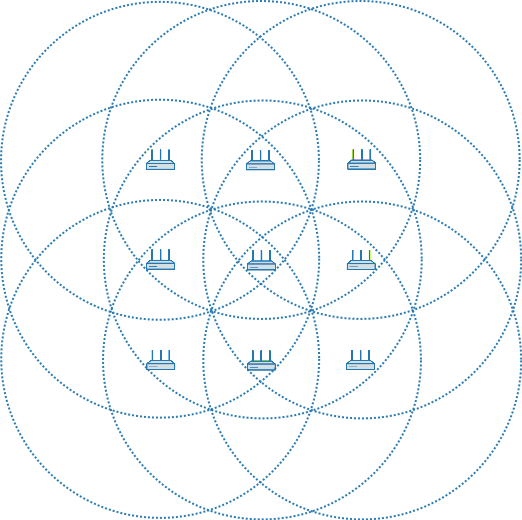
\includegraphics[width=0.39\columnwidth]{figures/3x3ap_range}
      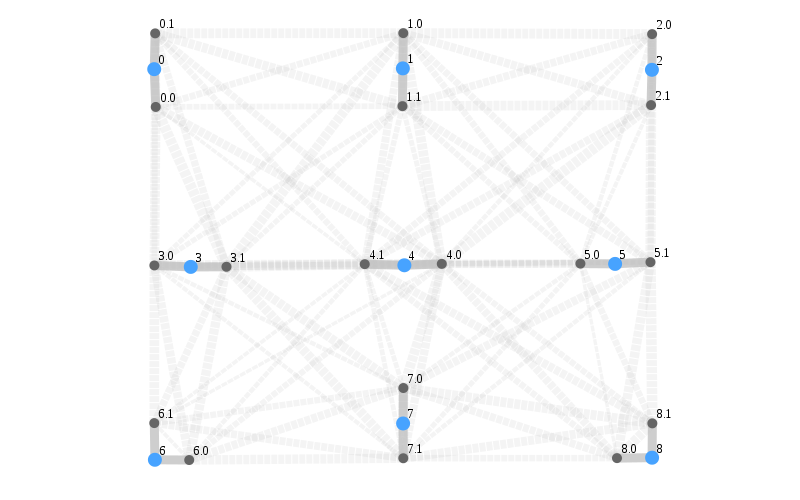
\includegraphics[width=0.6\columnwidth]{figures/3x3seen}
      \caption{Grid layout with two radio modules per \ac{AP} (left). Resulting network topology (right). Thicker edges indicate higher link-SNR.}
      \label{fig:3x3initial}
    \end{figure}
    
    \begin{figure}[h!]
      \centering
      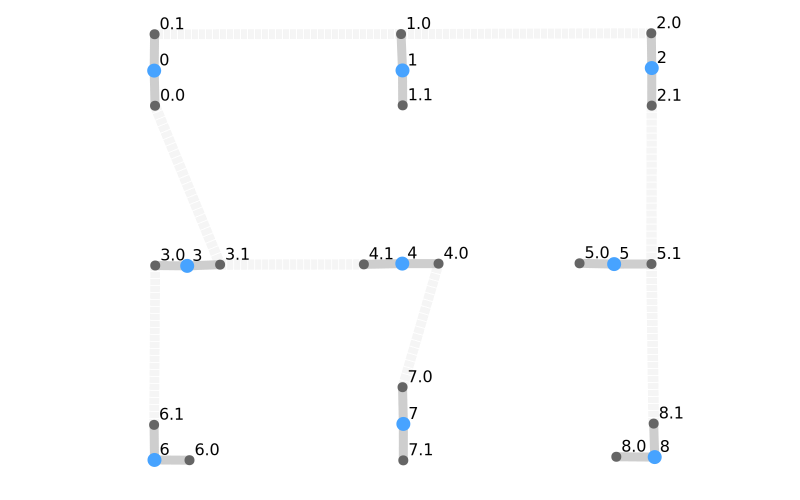
\includegraphics[width=0.49\columnwidth]{figures/3x3mst}
      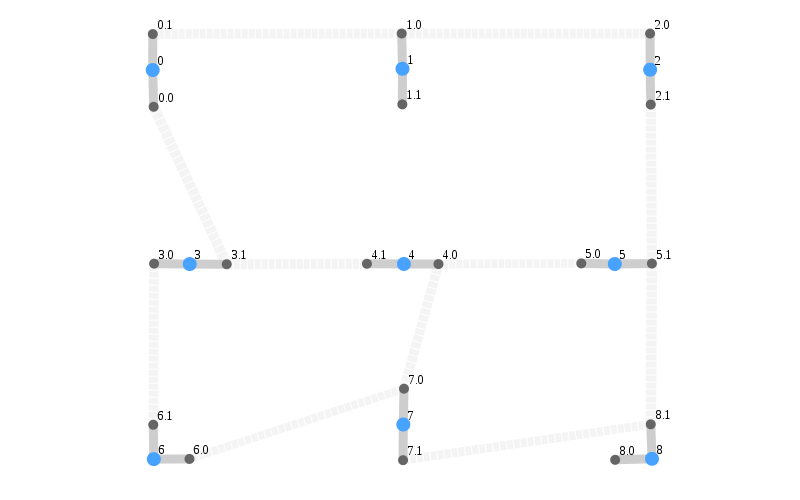
\includegraphics[width=0.49\columnwidth]{figures/3x3robust}
      \caption{Spanning tree on the graph(left) and spanning tree with survival paths(right)}
      \label{fig:3x3second}
    \end{figure}
    
    \begin{figure}[h!]
      \centering
      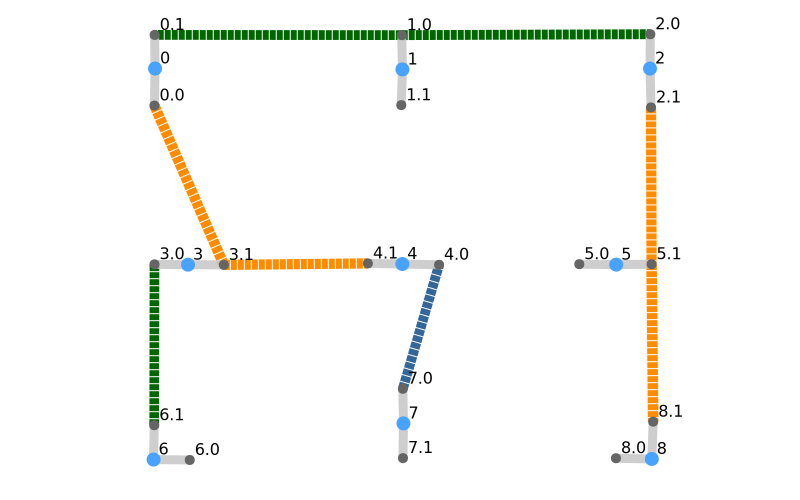
\includegraphics[width=0.49\columnwidth]{figures/3x3_ca_mst}
      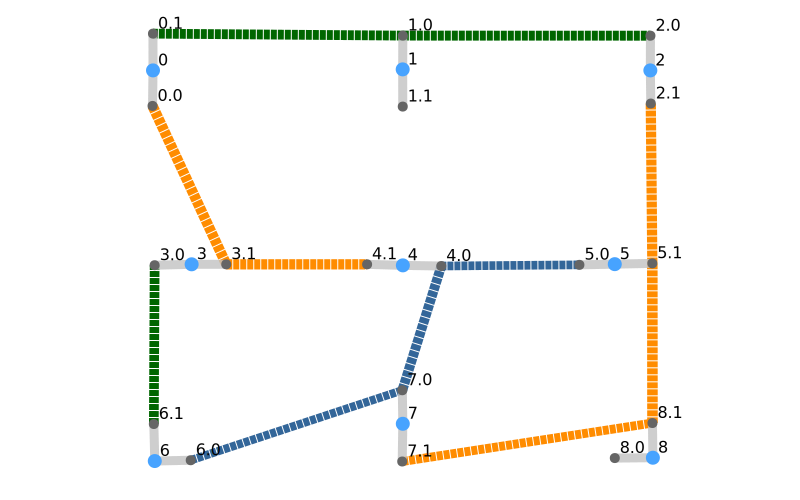
\includegraphics[width=0.49\columnwidth]{figures/3x3_ca_robust}
      \caption{Spanning tree with channels assigned(left) and spanning tree with survival paths with channels assigned(right)}
      \label{fig:3x3third}
    \end{figure}
    
    \newpage
  
  \section{Problems and Aids}
    \begin{description}
    \item [AutoWDS Status Tool:]
	To make things easier for debugging and also to actually see what is going on during the execution of the algorithms,
	we and most of all my Christoph Wollgarten created a tool called AutoWDS, which is based on \cite{d3js}. 
	Furthermore attached with a tool to extract data from the WLC, it is able to display current statuses and established links of a deployed network.
	
	It works by reading a graph represented as a \ac{JSON}-file and displays it interactively in html with javascript.
	As it is basically a force directed graph, the nodes position themselves according to their SNR-edge-values. 
	Additionally you can drag and position single nodes freely anywhere on the map for better singularization of entities.
	In the tcca module we also included an export function called "write\_json(graph, filename)" which creates a json file to be read by the autowdsstatus tool.
	This tool has also been used to create most of the images in this thesis.
	
    \item [Representation of Tables in LANCOM Devices:]
	While writing the code which deals with the WLC and receives the data, we initially had some difficulties extracting the data out of the tables represented in the WLC since
	they reside there in a somewhat obscure format and are spread over different tables. So that we effectively had to gather the data and join them so that we receive a
	nice tables like \ref{tab:wlc} we can work with. Nevertheless we were able to cope with it, although the code for it is somewhat longer and cumbersome.
	
      \item [Python Logging Module:]
	Another great helper turned out to be the utilization of pythons logger module. We excessively made use of its Error/Warning/Info/Debug statements which made debugging
	a lot easier without being an obstacle if we did not need the output as we could just switch to a different level of logging and enjoy the silence.
    \end{description}

    \begin{figure}[h]
      \centering
      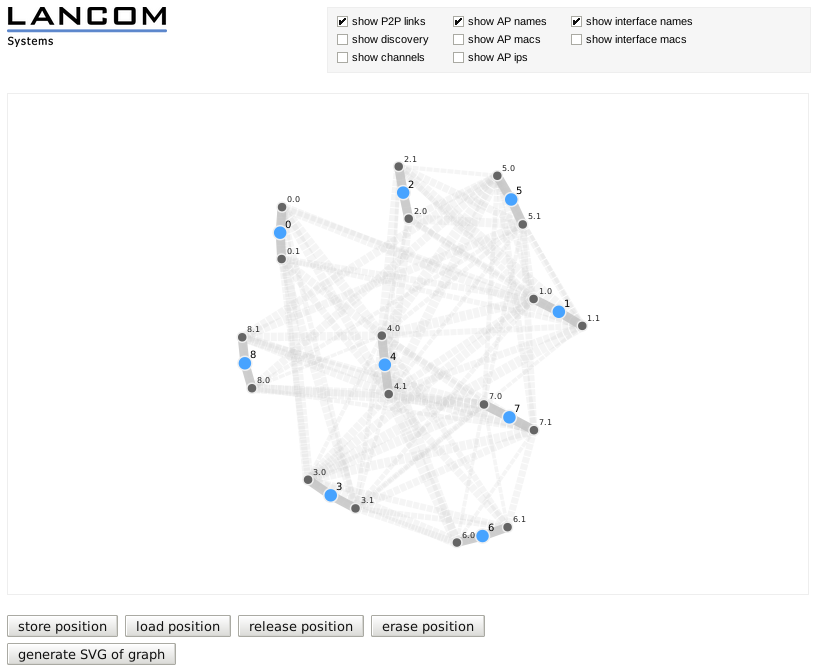
\includegraphics[width=0.85\columnwidth]{figures/autowdsstatus}
      \caption{AutoWDS status webinterface showing a network topology}
      \label{fig:autowdsstatus}
    \end{figure}
  
\clearpage

  

\chapter{Evaluation}
The goal of this paragraph is to assure that the changes we made to AutoWDS basic actually improved its performance.
Due to extent this work is aimed at, it was not feasible to implement all the systems of the related solutions on this field on a common environment
to get a fair assessment for each work. For this the overview papers on this area like \cite{overview_caa} may serve its purpose.
The following subsections will mainly focus on the comparison between AutoWDS basic and the extended version. Also we were not able to evaluate the performance gains
of some metrics like the survival path feature since the current implementation of AutoWDS only uses network bridges to connect the networks and no real routing infrastructure.
Due to this restriction only we are limited to spanning trees for the network since otherwise the STP would force shutdown the redundant links to eliminate
circles in the topology.
\section{Test Arrangement}
Since the main goal is to increase overall throughput performance as described in the requirements analysis, our basic evaluation approach is
to find by how much we were able to increase this metric. Therefore we ran both systems under equal circumstances with various settings and multiple runs
and compared its capacities.
  \subsection{Physical Infrastructure}
    For the test arrangement we used the following hardware:
      11 Accesspoints, 1 WLC and 2 Switches among those
      \begin{itemize}
       \item 3 x Lancom L322agn dual Wireless \cite{lancom}
       \item 3 x Lancom L-452agn dual Wireless
       \item 6 x Hirschmann OpenBAT-R
       \item 1 x Lancom WLC-4100
       \item 2 x Lancom GS-2352P
      \end{itemize}
      running on Firmware Version 9.0. We deployed them at a typical office environment as depicted in the figure.
      Only omnidirectional antennas for the accesspoints were used for this setup. As we had to connect each of the accesspoints also
      per cable to the monitoring station and power grid in order to route traffic through them and the network they're spanning,
      we could not set them further apart.
      Increasing the distance between the single APs would have lead to a sparser network topology and so the hidden station problem would have occured
      more often. Thus the actual interference would have gone up, since with a lower Signal to Noise ratio the APs would not be able to recognize each others 
      transmissions as those and categorize it as interference instead of applying CSMA/CD, leading to more corrupt packets.
      We were able to simulate this problem with a reduced transmit-power,
      but even on the lowest setting most of the accesspoints were able to receive each others beacons. With this limitation kept in mind we expect
      the gap between the two scenarios in the following results to be even greater.
      Since this test was conducted at a research facility for wireless LAN devices, especially the 2.4Ghz band was quite heavily utilized as you will notice
      in the performance charts.
    \begin{figure}[t]
      \centering
      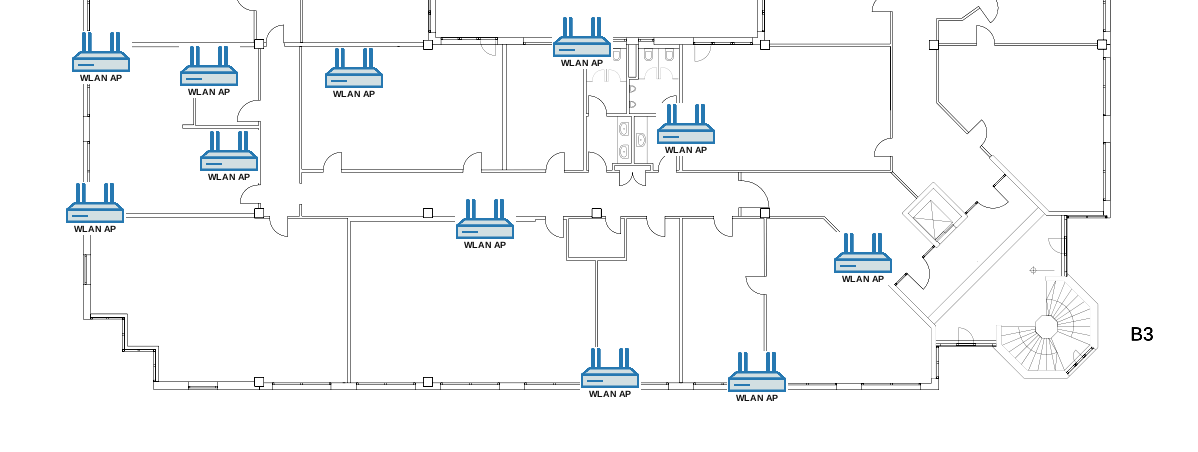
\includegraphics[width=1\columnwidth]{figures/Lancom-flur-withaps}
      \caption{Physical arrangement of accesspoints in a typical office complex spread over an area of rougly 15m x 40m}
      \label{fig:2ndfloor}
    \end{figure}
  \subsection{Network Infrastructure}
    \begin{figure}[h]
      \centerline{
	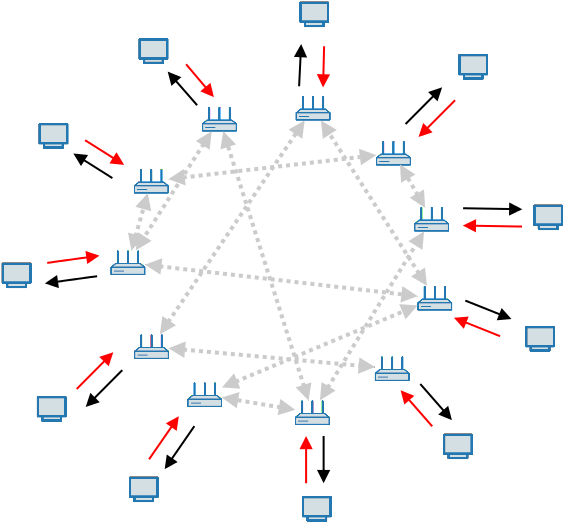
\includegraphics[width=0.3\textwidth]{figures/testsetup_logic}
	\caption{Example for the logical arrangement of accesspoints with systems attached by cable, which generate broadcast traffic that is routed through the 
	wireless network spanned by the accesspoints.}
      }
      \label{fig:testsetup_logic}
    \end{figure}
    The basic approach for measuring the throughput is to attach traffic generators to the accesspoints and make those send as much broadcast traffic to all
    other stations which are part of this network and therefore saturate the throughput capabilities of the network.
    \begin{figure}[h]
      \centerline{
	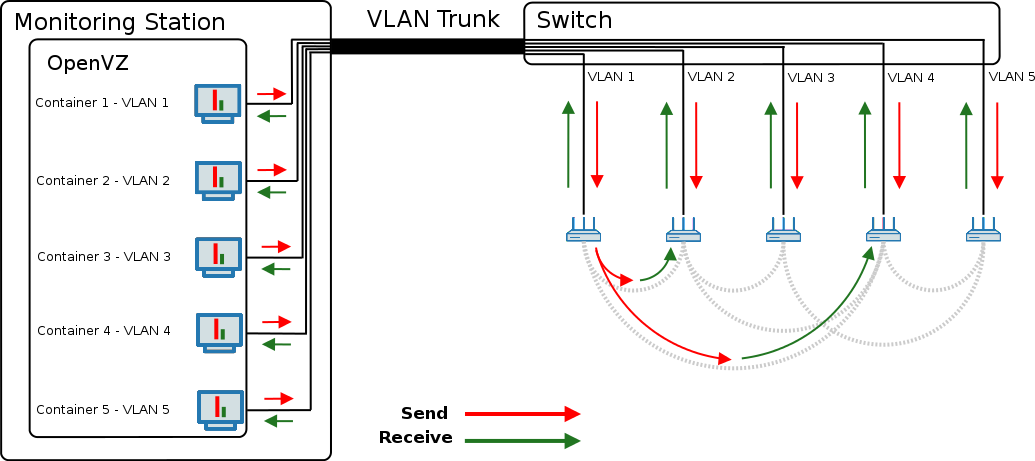
\includegraphics[width=0.6\textwidth]{figures/testsetup_openvz}%
	\caption{Implementation of the test arrangement with available hardware.}
      }
      \label{fig:testsetup_openvz}
    \end{figure}
    We simulated the traffic generating systems with OpenVZ \cite{openvz} on one Host with a VLAN for each system. The VLAN infrstructure is completely transparent
    to the VZ containers and the accesspoints since the monitoring stations encapsulates all frames before sending if over the VLAN Trunk to the switch, which again 
    decapsulates the frames before sending them to the accesspoints.
    To generate the traffic we used IPerf \cite{iperf} on the attached systems in UDP mode with a datarate of 1Mbit per second for a total of 10 Minutes.
    Since we could not directly send UDP frames to broadcast addresses with iperf, we ran multiple instances of iperf with different target ip addresses.
    Although 1Mbit for each stream may not seem much, but after multiplying it with the number of targets and the up- and downstreams the effective rate results in
    1Mbit * 12 * 2 = 24Mbit/s for each accesspoint. As we will see later on this will turn out to be enough to completely saturate the wireless network but still within
    the capabilities of the used Gigabit Ethernet to get the data to the accesspoints, as 24Mbit/s * 11 = 264Mbit/s does not exceed the 1000Mbit/s VLAN Trunk connection
    as possible bottleneck.
    \begin{listing}[t]
      \begin{lstlisting}
iperf -u -c 172.16.40.2* -t 600 -b 1M
      \end{lstlisting}
      \caption{IPerf's parameters to generate the traffic.}
      \label{lst:iperf}
    \end{listing}
\section{Metrics}
  \subsection{Test Duration}
     Each testcase was run for a total of 10 minutes as this should be enough to transgress any temporary effects. To get status snapshots we querried the accesspoints
     every 7 seconds for their state, which includes the bytes transferred and received so far. We did not query them more often since this could have 
     affected the accesspoints transfer performance as reading its internal tables and sending the results back means additional stress.
  \subsection{Channelusage}
    For AutoWDS basic we configured the Accesspoints to only use the following sets of Channels:
    \begin{itemize}
     \item 1 (2.4 GHz only)
     \item 36 (5GHz only)
    \end{itemize}
    For the extended version of AutoWDS we used the following channels as input for the allocation algorithm: 
    \begin{itemize}
     \item 1,6,11 (2.4 GHz only)
     \item 36,40,44 (5GHz only)
     \item 1,6,11,36,40,44 (2.4/5 Ghz mixed)
    \end{itemize}
    
    \begin{figure}[h]
      \centerline{
	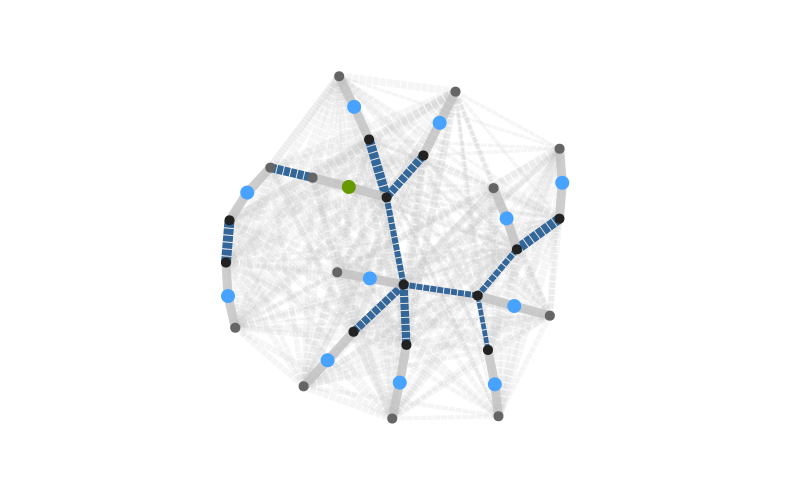
\includegraphics[width=0.7\textwidth]{figures/topo_chan_1}%
	\caption{Topology of the testnetwork with only channel 1 used. Different colors indicate different channels}
      }
      \label{fig:topo_chan_1}
    \end{figure}
    
    \begin{figure}[h]
      \centerline{
	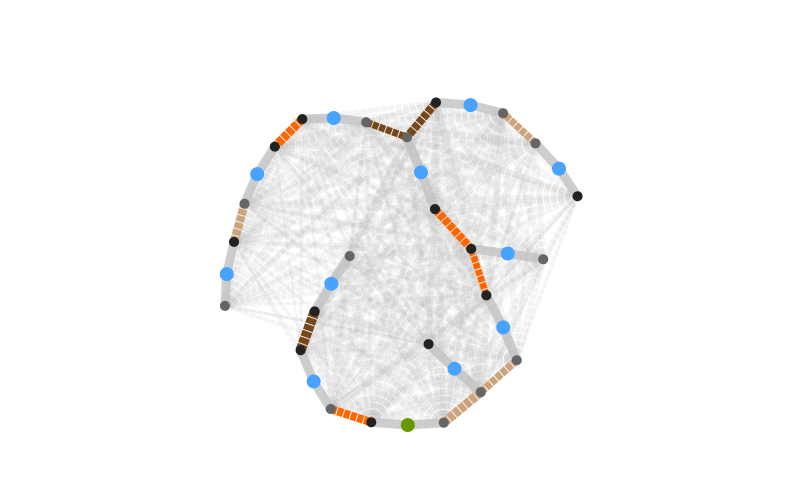
\includegraphics[width=0.7\textwidth]{figures/topo_chan_36_40_44}%
	\caption{Topology of the testnetwork with only channel 36,40,44 being used.}
      }
      \label{fig:topo_chan_36_40_44}
    \end{figure}

    \begin{figure}[h]
      \centerline{
	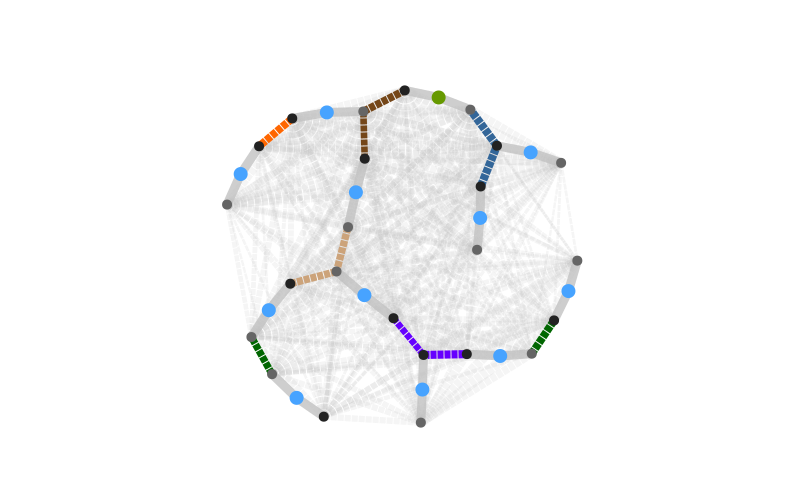
\includegraphics[width=0.7\textwidth]{figures/topo_chan_1_6_11_36_40_44}%
	\caption{Topology of the testnetwork with only channel 1,6,11,36,40,44 being used.}
      }
      \label{fig:topo_chan_1_6_11_36_40_44}
    \end{figure}
    
    \subsection{Characteristics}
    Due to the exceptional utilization of the 2.4 Ghz band in the area around the test arrangement, we had to carefully chose time and day
    for running the tests. We noticed a significant drop in radio usage for weekends and evenings and were able to schedule our tests in those timeframes.
    We additionally ran the testcases with two different settings to simulate the hidden station problem. Therefore we first set the radios to full power 
    resulting in a high connectivity between the nodes and on a second run decreased the transmit power as much as possbile to get a network with a smaller degree
    of interconnectivity.
\section{Results}
  \subsection{Expectations}
    We would expect a significant increase of data that has been able to transmit due to the usage of multiple collision domains the same one could
    expect by comparing a network hub, which has essentially just one collision domain and a network switch which has multiple domains and does not have
    to wait until the medium is free for sending again. The second source for an increased throughput would be the number of packets that could be received
    without errors due to interference.
  \subsection{Actual Results}
    
    \begin{figure}[h]
      \centerline{
	\includegraphics[width=0.62\textwidth]{figures/TestDataDiagramme/20/rx_bytes}%
	\includegraphics[width=0.38\textwidth]{figures/TestDataDiagramme/20/rx_bytes_boxplot}%
	\caption{Received bytes with decreased antenna transmit power}
      }
      \label{fig:rx20_bytes}
    \end{figure}
    
    \begin{figure}[h]
      \centerline{
	\includegraphics[width=0.62\textwidth]{figures/TestDataDiagramme/3/rx_bytes}%
	\includegraphics[width=0.38\textwidth]{figures/TestDataDiagramme/3/rx_bytes_boxplot}%
	\caption{Received bytes with full transmit power}
      }
      \label{fig:rx3_bytes}
    \end{figure}
    
    \begin{figure}[h]
      \centerline{
	\includegraphics[width=0.56\textwidth]{figures/TestDataDiagramme/3/recpackerr}%
	\includegraphics[width=0.44\textwidth]{figures/TestDataDiagramme/3/recpackerr_boxplot}%
	\caption{Ratio of successfully received packets to packets containing errors for reduced transmit power scenario}
      }
      \label{fig:3recpackerr}
    \end{figure}
    
    \begin{figure}[h]
      \centerline{
	\includegraphics[width=0.56\textwidth]{figures/TestDataDiagramme/20/recpackerr}%
	\includegraphics[width=0.44\textwidth]{figures/TestDataDiagramme/20/recpackerr_boxplot}%
	\caption{Ratio of successfully received packets to packets containing errors for full transmit power scenario}
      }
      \label{fig:20recpackerr}
    \end{figure}
    
    The results perfectly match our expectations. They also confirm that the 5Ghz band is superior to the 2.4Ghz with respect to throughput and reliability.
    We used the following channel sets for the actual implementation:
      
    \subsubsection{Assessment of AutoWDS basic}
      Using only a single channel for each wireless link does not scale very well in either of the two power setups, independent of the band used (2.4Gz or 5Ghz).
      Although the 5Ghz channels perform a little better in the high power setup, there seems no recognizable difference for the low power scenario.
      TODO: Explain why 5Ghz better in this scenario.
      Also with an increased transmit-power the number of packets which contain errors increases dramatically from an average of 10 percent to an average of 
      65 percent. TODO: How to explain this?
      Surprisingly the error rates for the 5Ghz channels already start high but seem to increase less than the 2.4Ghz channels.
      The results also affirm our estimate that the current version is not capable of transferring a little more than the control data.
      While setting up our test environment we also noticed that this effect of medium overload is no result of the size of our network.
      Whereas two unimpeded accesspoints were able to achieve a throughput of about 2Mbit in each direction, adding a third one would dramatically 
      decrease overall throughput down to about 100kbit or less, growing worse with each newly added accesspoint in receive-range. Even spreading the 
      accesspoints further apart would not promise better results since the inhering problem of using the same channel for the forwarding and receiving 
      link restricts the forwarding capabilities rigorously.
    \subsubsection{Assessment of AutoWDS extended}
      As the figures show, the outcome is dependent on the number of channels used as a setup with only 3 distinct channels allowed yields still better
      results than a mono-channel-setup but is inferior to a setup where we can use more channels as this gives us the possibility to use more collision domains
      which results in a higher available bandwidth and therefore increased throughput. In our example we used accesspoints with only two radios equipped, which
      limits us in selecting separate modules for different connections so that an accesspoint which already established two connections over its two modules
      would have to share one of its modules in order to apply a new link to a foreign accesspoint in order to maintain connectivity.
      \begin{figure}[h]
	\centerline{
	  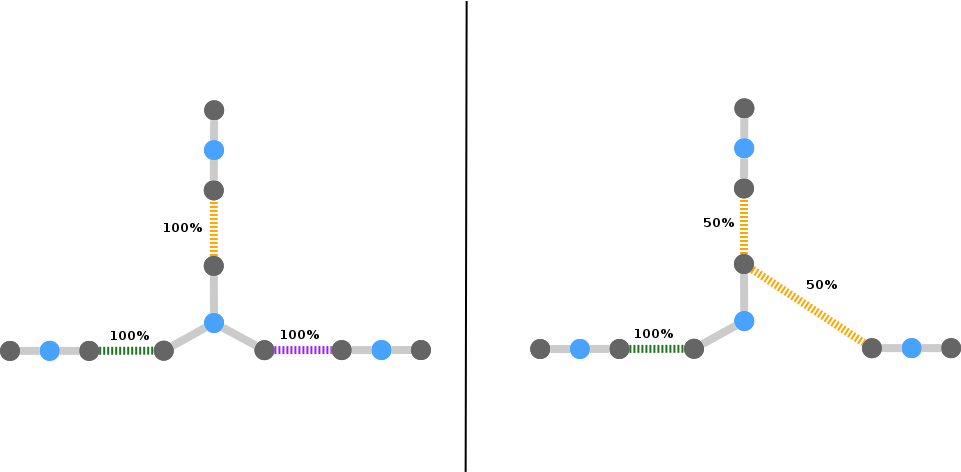
\includegraphics[width=0.56\textwidth]{figures/3modulesvs2}%
	  \caption{Link separation capability for an accesspoint with 3 modules compared to an accesspoints with 2 modules.}
	}
	\label{fig:3modulesvs2}
      \end{figure}
      Compared to the base scenario our link selection and channel assignment algorithm was able to double the throughput with every channel added. Of course this
      effect is limited by using a separate channel for each link and also by the number of modules for an accesspoint 
      since the former effectively assigns each link its own private channel and the latter is a question of practical relevance as current accesspoints are only 
      shipped with 2 or a maximum of 3 radio modules. As our gathered data indicate it is obviously an improvement to utilize multiple channels and modules
      compared to the basic AutoWDS, but in how far our solution comes in range of a theoretical optimal solution for a given scenario is still a question to be
      answered.
\section{Reflection on the Requirements}
  How far does the solution meet the requirements?\newline
  \subsection{Increased Throughput}
    Our measurement results indicate that throughput could significantly be increased. How much is determined by the input parameters of the algorithms like
    channels that can be utilized and hardware environments like the number of radio modules available at the accesspoints. 
  \subsection{Reduced Connectivity Failures}
    The survival path property takes care of this requirement. That is for the given error-scenario of one failing connection at a time, there is always
    a backup connection over a different link available as far as the underlying topology permits. As we were not able to test this feature 
    with the given implementation we are nevertheless confident that also this requirement has been met.
    If multi-flow / routing support will be implemented for our hardware in the future a decrease in node separation for failing links should be recognizable.
    Therefore we also met the successfully met the requirement of a two-edge-connected network topology.
  \subsection{Multiple Radios Utilized}
    Our algorithm utilizes the radio-modules as far as they are relevant for creating links between accesspoints with a high estimated throughput.
    Depending on the given infrastructure not all radio modules are necessarily used, since not all of them are needed in order to create a connected network topology.
    Moreover using all available links would not be beneficial as the hop distance would decrease but the effective throughput would also decrease by a factor 
    more than the number of participants in that channel.       
    \begin{figure}[h]
      \centerline{
	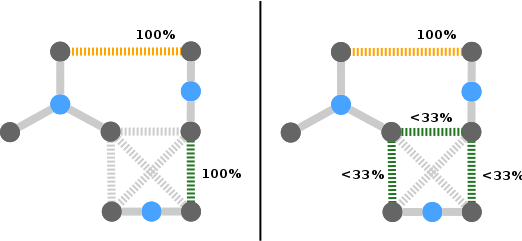
\includegraphics[width=0.56\textwidth]{figures/lessismore}%
	\caption{Due to the channel separation and exclusive access to one channel the left scenario is more favourable than the right, since throughput empirically
	exponentially decreases and is far below the 33 percent which those links would have to yield in order to at least provide the same throughput}}
      \label{fig:lessismore}
    \end{figure}
    In addition having some radio modules to spare gives us the opportunity to use those for client connections and assigning them a channel which does not interfere with the
    wireless backbone.
    \begin{figure}[h]
      \centerline{
	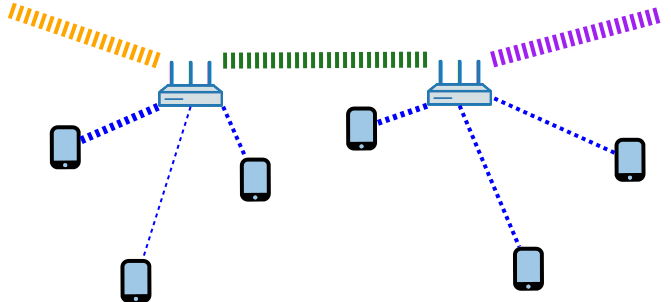
\includegraphics[width=0.56\textwidth]{figures/moduletospare}%
	\caption{Unused Modules used for separate client connections without interfering wlan backbone}
      }
      \label{fig:moduletospare}
    \end{figure}
  \subsection{Solution Works Within the Perimeter}
    The requirement dictates that computing a solution should be possible on a centralized entity (Servers/WLC).
    Our algorithm was implemented as a python script and can be run on a single system if given the right input data.
    Also the second requirement is fullfilled, since our algorithm is specially designed for a static environment where link quality and linkstate stay the same
    for a foreseeable time. If major changes in network connectivity or link quality occur the chosen network topology and channel assignment
    may lead to suboptimal results, therefore also a recomputation of the network topology has to be triggered.
    Currently there are no automatic triggers implemented, but planned in the future.
  \subsection{Comply with Economic Restrictions}
    The Runtime of the algorithms is mainly dependent on the number of connections between the nodes. Calculating the initial spanning tree is done in BFS mode and 
    therefore has quadratic runtime for the worst cast, depending on how sparse the graph is. The following calculation of the survival paths has also quadratic runtime 
    since we iterate over all connections and for each connection in the worst case over all other connections to find the backup path. The channel assignment is then again
    In a common deployment scenario the underlying network graph will be very sparsly connected since the number of accesspoints used and placement are carefully selected.
    Mostly they are placed in a way that they span a network over an area as far as possible.
    Current deployments and deployments in near future won't exceed 100 accesspoints. Even if fully meshed with a total of \(\sum \limits_{i=1}^{100} i = \frac{100(100+1)}{2}=5050\)
    edges it won't pose a problem to the capabilities of a WLC or an administrators machine.
  \subsection{Utilize Variable Number of Radios}
    As requested our algorithm selects channels from a given input set of channels. Only those channels are then used to determine the channel assignment.
    It is even possible to specify only one channel, resulting in a topology optimized network graph only.
\section{Reflection on Related Work}
  Comparing our solution to those of others would need some common ground. For example hardware requirements, number of modules and in general heterogenity/homgenity of
  the network are factor that could play in favor of some algorithms and therefore won't lead to fair results. Additionally different solutions were designed to 
  achieve different goals like throughput, latency or weighted throughput networks. Certainly there we could agree on this common deployment and compare each solution for random
  networks with respect to throughput, but this would require a full-scale simulation as hardware-resources are limited and too easily prone to real world difficulties.
  Although maybe a key aspect of this work, we did not have enough time to simulate even our own solution and therefore neither those of others. Nevertheless we would appreciate
  if someone further work on this field. In order to at least provide some kind of comparison we take a look at the features of each solution.
  \subsection{Features of Related Work Systems}
    TODO:
  \subsection{Features of Our System}
    TODO:
\chapter{Conclusion}
  In this work we have presented a new algorithm, which optimizes overall throughput of a \ac{WDS} by evading interference through an optimized network topology 
  and utilizing multiple channels with multiple radios. Additionally it creates a more failure resistant network topology by adding redundant links to the infrastructure.
  
  We implemented this algorithm in python to make this approach easy to use, customizable and comprehensible by providing examples, 
  explanations for how and why we did things the way we did and documenting our code.
  
  Our evaluation indicates a major improvement on the existing AutoWDS basic of at least up to 9 times the throughput in an admittedly rather small testbed.
  Yet, the optimization made the system really usable for wireless clients with high throughput demands.
  
  Although this work does not break any new ground in scientific research, it solves the imposed problem well by reusing and extending existing ideas and algorithms to
  achieve its goal of considerably increasing throughput for a given \ac{WDS}.
  
  \section{Limitations}
    The requirements analysis explicitly dictates the static attribute of APs and consequently their link quality, therefore our solution won't yield good 
    results for more volatile setups where link quality or network topology change frequently as the topology is not continuously optimized. 
    This would be the case if for example the APs are mobile or the environmental factors impacting link quality change rapidly and/or often.
    
    Since also a key requirement, this solution works only in a centralized managed fashion and thereby can't be used for unmanaged more autonomous APs.
    
  \section{Future Work}
    Open issues which could not be addressed by us, but nevertheless would like 
    to see implemented or tested are the following:
    \begin{description}
      \item [Further Evaluation:]
	Our evaluation is more a proof of concept instead of an elaborate audit. As described we ran our throughput-tests only in our lab environment, 
	which was also designed with other metrics and scenarios kept in mind. Therefore a more thorough and dedicated approach would include increased hardware diversity, 
	in general the full scale testing of up to 100 devices and longer test-periods with varying deployment parameters like transmit-power, 
	configuration timings and different topologies.
	Especially simulating our solution with random graph layouts and different underlying topologies could provide opportunities to even further increase throughput.
	Also the feature of evading foreign used channels should be evaluated if the implementation of 
	AutoWDS permits as this will be one of the factors which strongly affect performance.
      
      \item[Extensive Comparison to Related Work:]
	As we only compared our work by listing features, a true comparison still has to be done if one would 
	like to know the strength and weaknesses considering actual throughput-performance.
	As noted this will probably take some time as all the solutions would have to be 
	implemented in presumably the same language. And then deciding on the environmental settings
	like interference by other devices and node connectivity will create new challenges.
      
      \item[Further Optimization of the Algorithm:]
	Algorithm runtime is not in the focus of concern at the moment but could be in the future. 
	As a result and in order to more closely integrate the solution into AutoWDS extended,
	porting the code to a native language like C/C++ could give some additional performance gains.
      
      \item[Learning Algorithm:]
	In its current state, the optimization is triggered through the administrator or user during the initial setup or every now and then if
	the network appears slow. As this always just captures the status quo of the network, the optimization is susceptible to
	temporary interferences which could lead to suboptimal results in the long run and it would have to be rerun in order to keep up the best topology possible.
	To deal with the snapshot difficulty we had the idea of also looking at the history of a used channel and then decide if it would be worth it to continue
	to use a certain link and channel or switch to another one. 
	This would allow us to better evaluate link-quality and provide us with a more fine 
	grained view on the network as a whole and how it is affected by other influences over time. 
	We could then act upon those changes automatically in a more timely manner leading to even better results.
	
    \end{description}


%%%%%%%%%%%%%%%%%%%%%%%%%%%%%%%%%%%%%%%%%%%%%%%%%%%%%%%%%%%%%
%% LITERATUR UND ANDERE VERZEICHNISSE
%%%%%%%%%%%%%%%%%%%%%%%%%%%%%%%%%%%%%%%%%%%%%%%%%%%%%%%%%%%%%
%% Ein kleiner Abstand zu den Kapiteln im Inhaltsverzeichnis (toc)
\ifnotdraft{
\addtocontents{toc}{\protect\vspace*{\baselineskip}}
\cleardoublepage
%% Literaturverzeichnis
\phantomsection % phantomsection wird benötigt, damit z.B. hyperref die richtige Seite verlinkt.
\addcontentsline{toc}{chapter}{Bibliography}
%\nocite{*} %Auch nicht-zitierte BibTeX-Einträge werden angezeigt.
\bibliography{literature/literature}%Eine Datei 'literatur.bib' wird hierfür benötigt.
\bibliographystyle{styles/acmurl}%Art der Ausgabe: plain / apalike / amsalpha / ...
}

%% Abbildungsverzeichnis
%\clearpage
%\addcontentsline{toc}{chapter}{List of Figures}
%\listoffigures

%% Tabellenverzeichnis
%\clearpage
%\addcontentsline{toc}{chapter}{List of Tables}
%\listoftables


%%%%%%%%%%%%%%%%%%%%%%%%%%%%%%%%%%%%%%%%%%%%%%%%%%%%%%%%%%%%%
%% ANHÄNGE
%%%%%%%%%%%%%%%%%%%%%%%%%%%%%%%%%%%%%%%%%%%%%%%%%%%%%%%%%%%%%
\appendix
\chapter{Appendix}

\section{List of Abbreviations}

\begin{acronym}[ABCDEFGH]
	\setlength{\itemsep}{-\parsep}
        \acro{AP}{Accesspoint}
        \acro{AutoWDS}{Automatic WDS}
        \acro{BFS}{Breadth First Search}
        \acro{BFS-CA}{Breadth First Search Channel Assignment}
        \acro{CAA}{Channel Allocation Algorithm}
        \acro{CA}{Channel Assignment}
        \acro{CAPWAP}{Control And Provisioning of Wireless Access Points}
        \acro{CAS}{Channel Assignment Server}
        \acro{CCA}{Clustered Channel Assignment}
        \acro{CLICA}{Connected Low Interference Channel Assignment}
        \acro{CSMA/CA}{Carrier Sense Multiple Access / Collision Avoidance}
        \acro{CTA}{Centralized Tabu-based Algorithm}
        \acro{CTS}{Clear To Send}
        \acro{DJP}{Dijkstra, Jarník, Prim}
        \acro{DTLS}{Datagram Transport Layer Security}
        \acro{DVB-T}{Digital Video Broadcasting – Terrestrial}
        \acro{ESSID}{Extended SSID}
        \acro{HD}{High Definition}
        \acro{IDE}{Integrated Development Environment}
        \acro{IEEE}{Institute of Electrical and Electronics Engineers}
        \acro{INSTC}{Minimum Interference Survivable Topology Control}
        \acro{IP}{Internet Protocol}
        \acro{JSON}{JavaScript Object Notation}
        \acro{LAN}{Local Area Network}
        \acro{LCI}{Link Co-channel Interference}
        \acro{LCOS}{LANCOM Operating System}
        \acro{MAC}{Media Access Control}
        \acro{MCG}{Multi-Radio Conflict Graph}
        \acro{MPLS}{Multiprotocol Label Switching}
        \acro{MST}{Minimal Spanning Tree}
        \acro{MUP}{Multi-radio Unification Protocol}
        \acro{PAN}{Personal Area Network}
        \acro{PEP8}{Python Enhancement Proposal 8}
        \acro{RTS/CTS}{Request To Send / Clear To Send}
        \acro{RTS}{Request To Send}
        \acro{SHF}{Super High Frequency}
        \acro{SNMP}{Simple Network Management Protocol}
        \acro{SNR}{Signal-to-Noise Ratio}
        \acro{SSH}{Secure SHell}
        \acro{SSID}{Service Set Identifier}
        \acro{STP}{Spanning Tree Protocol}
        \acro{Telnet}{Telecommunication Network}
        \acro{TLV}{Type-Lenght-Value}
        \acro{UDP}{User Datagram Protocol}
        \acro{UHF}{Ultra High Frequency}
        \acro{VLAN}{Virtual Local Area Network}
        \acro{WDS}{Wireless Distribution System}
        \acro{WLAN}{Wireless Local Area Network}
        \acro{WLC}{Wireless LAN Controller}
        \acro{WMN}{Wireless Mesh Network}
        \acro{WPA2}{Wi-Fi Protected Access 2}
\end{acronym}


\end{document}
